\documentclass[a4paper,dvipdfmx]{jarticle}
\usepackage{caption}
% 数式用
\usepackage{amsmath, amsfonts}  % 数式用
\usepackage{bm} % 数式中の太字
\usepackage{amssymb} % 記号
% 画像用
\usepackage{float} % 画像の挿入箇所を固定
\usepackage[dvipdfmx]{graphicx} % 画像挿入用
\usepackage{wrapfig} % 画像の周りに本文を流し込み
% ページレイアウト
\usepackage{here} % 画像を強制的に出力
\usepackage{url} % URLリンク
\usepackage{hyperref} % 
\hypersetup{
  colorlinks=false, % リンクに色をつけない設定
  bookmarks=true, % 以下ブックマークに関する設定
  bookmarksnumbered=true, % ブックマークに節番号などをつけるか
  pdfborder={0 0 0}, % 枠なし
  bookmarkstype=toc % 目次情報のブックマークを作る
}
\usepackage{multirow} % 表で行結合
\usepackage[margin=20truemm]{geometry} %余白調整
% 文字装飾
\usepackage{color} % 文字色
\usepackage[table,xcdraw]{xcolor} % 表の色
\usepackage{ascmac} % 丸枠
\usepackage{fancybox} % 丸枠
\usepackage{booktabs} % 表の横線を調整するためのパッケージ
\usepackage{tabularx} % 表の幅を調整するためのパッケージ
\usepackage{tcolorbox} %ボックスやフレームを作成するためのパッケージ

\begin{document}
\begin{titlepage}
  \centering
  \LARGE
  内部設計書
  \\\vspace{3cm}
  地域密着型アルバイト求人アプリ\\
  \textbf{REEL(Region Event Excitement Linkup)}
  \\\vspace{4cm}
  第 1.0 版
  \\\vspace{4cm}
  \today
  \\\vspace{2.5cm}
  \textbf{ChaO!株式会社}
\end{titlepage}
\tableofcontents
\newpage
% 概要はabstract
% 動作環境はrequirements
% 開発環境はdevelopment
% コーディング規約はcoding
% モジュール設計はmodule
% API設計はapi
% データベース設計はdatabase
% メンバの貢献度はcontribution
\section{概要}
この文書は、REELアプリケーションの内部設計について記述したものである。

\section{動作環境}
本アプリケーションREELは以下の環境で動作することを想定している。
\begin{itemize}
  \item iOS
  \item Android
\end{itemize}
ウェブアプリケーションとしての動作は想定していない。
\section{開発環境}
\section{コーディング規約}
\subsection{Dart}

\subsection*{識別子}
Dartの識別子には以下のように大きく３種類に分けることが出来る。\par
\begin{itemize}
  \item \textbf{UpperCamelCase}：名前では、各単語の最初の文字が大文字になり、最初の文字も含まれる。
  \item \textbf{lowerCamelCase}：名前では、頭文字を覗き、各単語の最初の文字を大文字にする
  \item \textbf{snake\_case}：頭字語であっても、小文字のみを使用し、単語は\_で区切る。
\end{itemize}
これを元に型やファイルなどの識別子を定める。

\subsubsection*{・型にはUpperCamelCaseを用いる。}
クラス、列挙型、typedefs、型パラメータは、各単語の最初の文字を大文字にし（最初の単語を含む）、セパレータを使用しない。\par
これには、メタデータ注釈で使用されることを意図したクラスも含む。\par

アノテーションクラスのコンストラクタがパラメータを取らない場合、それ用に別のloweCamelCase定数を作成した方が良い。\par

\subsubsection*{・拡張子には、UpperCamelCaseを使う。}
タイプ同様、拡張子は各単語の最初の文字を大文字に（最初の単語を含む）、セパレータを使用しない。\par





\subsubsection*{・ライブラリ、パッケージ、ディレクトリ、ソースファイルにはsnake\_caseを使う}
ファイルシステムによっては大文字と小文字が区別されないため、
多くのプロジェクトでファイル名を全て小文字にする必要がある。
区切り文字を使用することで、
そのような形式でも名前を読むことができる。
アンダースコア（\_）をセパレータとして使用すると、
名前が有効なDart識別子であることが保証される。これは、
言語が後にシンボリックインポートをサポートする場合に便利である。\par

\subsubsection*{・インポートプレフィックスにはsnake\_caseを使う}
\ \par

\subsubsection*{・他の識別子（変数名や関数名）にはlowerCamelCaseを使う}
クラスメンバー、トップレベル定義、変数、パラメータ、
名前付きパラメータは、
最初の単語を除く各単語の最初の文字を大文字にし、
セパレータを使用しない。\par
\clearpage

\subsubsection*{・定数には、lowerCamelCaseを使う方が良い}
新しいコードでは、enum値を含む定数変数にlowerCamelCaseを使用する。\par

次の場合のように、
既存のコードとの一貫性のためにSCREAMING\_CAPSを使用できる。\par
\begin{itemize}
  \item[$\blacktriangleright$]SCREAMING\_CAPS既に使用しているファイル
        またはライブラリにコードを追加する場合\par
  \item[$\blacktriangleright$]Javaコードと並行するDartコードを生成する場合、
        例えば、protobufsから生成された列挙されたタイプで
\end{itemize}



\subsubsection*{・3文字以上の頭文字と略語は1文字目を大文字にする（普通の単語のように扱う）}
\ \par



\subsubsection*{・未使用のコールバック引数には\ 、や\ \_\ を使用した方が良い}
\begin{itemize}
  \item[-] 関数に複数の未使用のパラメータがある場合は、
        名前の衝突を避けるために追加のアンダースコア（\_）を使用する。
\end{itemize}
\ \par


\subsubsection*{・プライベートではない識別子はアンダースコア（\_）から始めない}
\ \par
\subsubsection*{・インデント}
\begin{itemize}
  \item[-] 2スペース\par

  \item[-] 継続インデントは、4スペース\par


\end{itemize}
\ \par

\subsubsection*{・空行のインデント}
\ \par

\subsubsection*{・改行}
\begin{itemize}
  \item[-] 空行の場合はインデントを維持しない（スペースを削除する）\par

  \item[-] 引数が2つ以上のWidgetは複数行で書く\par

  \item[-] Widgetの引数が1つでも、その子Widgetが複数行の場合は、改行。
        （1行でWidgetを書くのは、Widgetツリーの末端のみ）\par

  \item[-] 例外として、Edgelnsetsは複数の引数があっても１行で良い\par

\end{itemize}
\ \par

\subsubsection*{・括弧の位置}
\begin{itemize}
  \item[-] 括弧の終了は、括弧の開始の後に改行しない場合は、同じ行で閉じる。\par


  \item[-] 括弧の開始の後に改行した場合、
        中身の最終行の次の行で括弧を閉じる。
        尚、インデントはブロック開始時と同じにする。\par


  \item[-] 関数の呼び出しで「名前なし引数」で開始する場合、
        同じ行でWidgetの括弧を開始する。
        Widgetの閉じる括弧と関数呼び出しの閉じる括弧は同じ行。\par

  \item[-] 関数の呼び出しで「名前あり引数」の場合は、
        Widgetと同様に記述。\par

\end{itemize}
\ \par
\clearpage

\subsubsection*{・コメント}
\begin{itemize}
  \item[$\blacktriangleright$] \verb|//|\ を使用
  \item[$\blacktriangleright$] コメント開始\ \verb|//|\ とコメント本文のは半角スペースひとつ開ける
\end{itemize}\par
\ \par


\subsubsection*{・クラス}
\begin{itemize}
  \item[-] new \verb|/| const\par
        オブジェクト生成時の new は省略する。 const は省略しない。\par


  \item[-] var \verb|/| final\par
        初期化値の代入以後で変更（再代入）しない変数は、
        final で宣言する。\par

\end{itemize}
\ \par
\subsubsection*{・三項演算子}
\begin{itemize}
  \item[-] 2つの値のどちらかを得るだけの場合など、
        単純な場合は使用して良い。
        結果にさらに式を含まないようにする。\par

  \item[-] 三項演算子のなかで使うものを予め計算するか、
        別にメソッドなどに切り分ける。\par

\end{itemize}



\ \par



\subsection*{順序}
\subsubsection*{・dart：から始まるインポートは他のインポートよりも前に置く}



\subsubsection*{・package：から始まるインポートは相対的なインポートよりも前に置く}


\subsubsection*{・エクスポートはインポートとは別のセクションで指定する＞}


\subsubsection*{・インポートやエクスポートは辞書順に並べ替える＞}
\ \par



\subsection*{整形}
\subsubsection*{・1行が81文字以上になることを避ける}

\subsubsection*{・ifやforの\{\}を省略しない}


\verb|-|例外として、ifにelseがなく、
かつ、全てが1行に収まる場合は{}は省略しても良い。\par
\ \par

\subsection*{・ツール}
コード作成時に自動でこれらのDart規約に従うように、
以下のツールを導入し調整を行う。\par
\begin{itemize}
  \item[-] VScodeの設定である”format on save”を有効化にし、自動的にフォーマットを行う
  \item[-] dart fix \verb|--|applyでコーディング規約に沿うように変換を行うコマンド
  \item[-] flutter analyzeでコーディング規約違反の有無を表示するコマンド
\end{itemize}

\clearpage

\subsection{Python}\label{sec:python}
\subsubsection{命名規約}
\begin{table}[H]
  \centering
  \caption{Pythonの命名規約}
  \label{tab:code-python}
  \begin{tabular}{|c|c|c|} \hline
    対象     & ケース                & 例                \\ \hline \hline
    モジュール名 & snake\_case        & database\_models \\ \hline
    パッケージ名 & snake\_case        & my\_package      \\ \hline
    クラス名   & UpperCamelCase     & UserCreate       \\ \hline
    関数名    & snake\_case        & create\_user     \\ \hline
    変数名    & snake\_case        & is\_active       \\ \hline
    定数名    & UPPER\_SNAKE\_CASE & THIS\_IS\_STATIC \\ \hline
  \end{tabular}
\end{table}
また、補足で"\_"で始まる変数は、プライベート変数を表し、外部からアクセスしないようにする。
例外クラスは、"Error"で終わるようにする。
インスタンスメソッドの第一引数は、"self"とする。
クラスメソッドの第一引数は、"cls"とする。
\subsubsection{コーディングスタイル}
コーディングスタイルは~\href{https://pep8-ja.readthedocs.io/ja/latest}{\textbf{PEP8}}~に従う。
また、意識せずともコーディングスタイルを統一するために、black Formatter,
isort, flake8を使用する。これらを保存時に自動で実行するように設定することで、
空行や改行、importの順番などを自動で整形する。

\clearpage
\section{モジュール設計}\label{sec:dart-module}

\subsection{overlay}

\begin{table}[H]
  \centering
  \begin{tabular}{|c|l|l|} \hline
    モジュール名 & \multicolumn{2}{l|}{rule\_screen.dart}  \\ \hline
    モジュール概要 & \multicolumn{2}{p{12cm}|}{利用規約のオーバーレイで表示される内容を生成するコンポーネント} \\ \hline
    責任者 & \multicolumn{2}{l|}{金川幸太} \\ \hline
    \multirow{7}{*}{構成要素} & クラス名 & RuleScreen      \\ \cline{2-3}
      & クラス種類 & OverlayEntry \\ \cline{2-3}
      & 処理概要 & \multicolumn{1}{p{12cm}|}{オーバーレイの内容を返す} \\ \cline{2-3}
      & 入力 & Buildcontext context, String text \\ \cline{2-3}
      & 出力 & Material \\ \cline{2-3}
      & \multicolumn{2}{l|}{他クラス・関数との関係}  \\ \cline{2-3}
      & \multicolumn{2}{p{14cm}|}{ボタンを押すことで、rule\_screen.dartのRuleScreen().show(context, text)が呼び出され、オーバレイ表示
      ElevatedButtonの処理がされると、RuleScreen().hide()によりcontrolle.closeが呼び出されオーバレイを閉じる}  \\ \hline
  \end{tabular}
\end{table}

\begin{table}[H]
  \centering
  \begin{tabular}{|c|l|l|} \hline
    モジュール名 & \multicolumn{2}{l|}{rule\_screen\_controller.dart}  \\ \hline
    モジュール概要 & \multicolumn{2}{p{12cm}|}{オーバーレイの表示、非表示の操作を行うコンポーネント}           \\ \hline
    責任者 & \multicolumn{2}{l|}{金川幸太}           \\ \hline
    \multirow{7}{*}{構成要素}  & クラス名 & RuleScreenControl      \\ \cline{2-3}
      & クラス種類 & immutable \\ \cline{2-3}
      & 処理概要 & \multicolumn{1}{p{12cm}|}{オーバーレイの内容を返す} \\ \cline{2-3}
      & 入力 & String text(option) \\ \cline{2-3}
      & 出力 & Widget \\ \cline{2-3}
      & \multicolumn{2}{l|}{他クラス・関数との関係}  \\ \cline{2-3}
      & \multicolumn{2}{p{14cm}|}{ CloseLoadingScreenによってオーバレイを閉じる \newline
      UpdateLoadingScreenによってオーバーレイを表示}  \\ \hline
  \end{tabular}
\end{table}

\subsection{provider}

\begin{table}[H]
  \centering
  \begin{tabular}{|c|l|l|} \hline
    モジュール名                & \multicolumn{2}{l|}{change\_general\_corporation.dart}                                                                   \\ \hline
    モジュール概要               & \multicolumn{2}{p{12cm}|}{アプリ全体で使用するプロバイダモジュール}                                                                          \\ \hline
    責任者                   & \multicolumn{2}{l|}{新谷光城}                                                                                                \\ \hline
    \multirow{7}{*}{構成要素} & クラス名                                                   & ChangeGeneralCorporation                                        \\ \cline{2-3}
                          & クラス種類                                                  & ChangeNotifier                                                  \\ \cline{2-3}
                          & 処理概要                                                   & \multicolumn{1}{p{12cm}|}{アプリ全体で使用する一般法人の判断を行うbool型変数、色を定義している。
    また、一般法人の値が変更されると、それに対応した色へと変更が行われる。}                                                                                                             \\ \cline{2-3}
                          & 入力                                                     & なし                                                              \\ \cline{2-3}
                          & 出力                                                     & なし                                                              \\ \cline{2-3}
                          & \multicolumn{2}{l|}{他クラス・関数との関係}                                                                                         \\ \cline{2-3}
                          & \multicolumn{2}{p{14cm}|}{なし}                                                                                            \\ \hline
  \end{tabular}
\end{table}

\begin{longtable}{|c|l|l|} \hline
      モジュール名                & \multicolumn{2}{l|}{app\_router.gr.dart}                                                          \\ \hline
      モジュール概要               & \multicolumn{2}{p{12cm}|}{RouteをRouterに変換するモジュール}                                                 \\ \hline
      責任者                   & \multicolumn{2}{l|}{新谷光城}                                                                         \\ \hline
      \multirow{7}{*}{構成要素} & クラス名                                              & \_\$AppRouter                                 \\ \cline{2-3}
                            & クラス種類                                             & extends\ RootStackRouter                      \\ \cline{2-3}
                            & 処理概要                                              & \multicolumn{1}{p{12cm}|}{MapにRouterを入れこむクラス} \\ \cline{2-3}
                            & 入力                                                & なし                                            \\ \cline{2-3}
                            & 出力                                                & Map                                           \\ \cline{2-3}
                            & \multicolumn{2}{l|}{他クラス・関数との関係}                                                                  \\ \cline{2-3}
                            & \multicolumn{2}{p{14cm}|}{app\_router.dartを組み込む}                                                  \\ \cline{2-3}
                            & クラス名                                              & HomeRouterRoute                               \\ \cline{2-3}
                            & クラス種類                                             & extends\ PageRouteInfo（void）                  \\ \cline{2-3}
                            & 処理概要                                              & \multicolumn{1}{p{12cm}|}{Routeの名前定義}         \\ \cline{2-3}
                            & 入力                                                & なし                                            \\ \cline{2-3}
                            & 出力                                                & なし                                            \\ \cline{2-3}
                            & \multicolumn{2}{l|}{他クラス・関数との関係}                                                                  \\ \cline{2-3}
                            & \multicolumn{2}{p{14cm}|}{なし}                                                                     \\ \cline{2-3}
                            & クラス名                                              & EventRouterRoute                              \\ \cline{2-3}
                            & クラス種類                                             & extends\ PageRouteInfo（void）                  \\ \cline{2-3}
                            & 処理概要                                              & \multicolumn{1}{p{12cm}|}{Routeの名前定義}         \\ \cline{2-3}
                            & 入力                                                & なし                                            \\ \cline{2-3}
                            & 出力                                                & Map                                           \\ \cline{2-3}
                            & \multicolumn{2}{l|}{他クラス・関数との関係}                                                                  \\ \cline{2-3}
                            & \multicolumn{2}{p{14cm}|}{なし}                                                                     \\ \cline{2-3}
                            & クラス名                                              & JobRouterRoute                                \\ \cline{2-3}
                            & クラス種類                                             & extends\ PageRouteInfo（void）                  \\ \cline{2-3}
                            & 処理概要                                              & \multicolumn{1}{p{12cm}|}{Routeの名前定義}         \\ \cline{2-3}
                            & 入力                                                & なし                                            \\ \cline{2-3}
                            & 出力                                                & なし                                            \\ \cline{2-3}
                            & \multicolumn{2}{l|}{他クラス・関数との関係}                                                                  \\ \cline{2-3}
                            & \multicolumn{2}{p{14cm}|}{なし}                                                                     \\ \cline{2-3}
                            & クラス名                                              & MyPageRouterRoute                             \\ \cline{2-3}
                            & クラス種類                                             & extends\ PageRouteInfo（void）                  \\ \cline{2-3}
                            & 処理概要                                              & \multicolumn{1}{p{12cm}|}{Routeの名前定義}         \\ \cline{2-3}
                            & 入力                                                & なし                                            \\ \cline{2-3}
                            & 出力                                                & なし                                            \\ \cline{2-3}
                            & \multicolumn{2}{l|}{他クラス・関数との関係}                                                                  \\ \cline{2-3}
                            & \multicolumn{2}{p{14cm}|}{なし}                                                                     \\ \cline{2-3}
                            & クラス名                                              & LoginRoute                                    \\ \cline{2-3}
                            & クラス種類                                             & extends\ PageRouteInfo（void）                  \\ \cline{2-3}
                            & 処理概要                                              & \multicolumn{1}{p{12cm}|}{Routeの名前定義}         \\ \cline{2-3}
                            & 入力                                                & なし                                            \\ \cline{2-3}
                            & 出力                                                & なし                                            \\ \cline{2-3}
                            & \multicolumn{2}{l|}{他クラス・関数との関係}                                                                  \\ \cline{2-3}
                            & \multicolumn{2}{p{14cm}|}{なし}                                                                     \\ \cline{2-3}
                            & クラス名                                              & HomeRoute                                     \\ \cline{2-3}
                            & クラス種類                                             & extends\ PageRouteInfo（void）                  \\ \cline{2-3}
                            & 処理概要                                              & \multicolumn{1}{p{12cm}|}{Routeの名前定義}         \\ \cline{2-3}
                            & 入力                                                & なし                                            \\ \cline{2-3}
                            & 出力                                                & なし                                            \\ \cline{2-3}
                            & \multicolumn{2}{l|}{他クラス・関数との関係}                                                                  \\ \cline{2-3}
                            & \multicolumn{2}{p{14cm}|}{なし}                                                                     \\ \cline{2-3}
                            & クラス名                                              & EventRoute                                    \\ \cline{2-3}
                            & クラス種類                                             & extends\ PageRouteInfo（void）                  \\ \cline{2-3}
                            & 処理概要                                              & \multicolumn{1}{p{12cm}|}{Routeの名前定義}         \\ \cline{2-3}
                            & 入力                                                & なし                                            \\ \cline{2-3}
                            & 出力                                                & なし                                            \\ \cline{2-3}
                            & \multicolumn{2}{l|}{他クラス・関数との関係}                                                                  \\ \cline{2-3}
                            & \multicolumn{2}{p{14cm}|}{なし}                                                                     \\ \cline{2-3}
                            & クラス名                                              & JobRoute                                      \\ \cline{2-3}
                            & クラス種類                                             & extends\ PageRouteInfo（void）                  \\ \cline{2-3}
                            & 処理概要                                              & \multicolumn{1}{p{12cm}|}{Routeの名前定義}         \\ \cline{2-3}
                            & 入力                                                & なし                                            \\ \cline{2-3}
                            & 出力                                                & なし                                            \\ \cline{2-3}
                            & \multicolumn{2}{l|}{他クラス・関数との関係}                                                                  \\ \cline{2-3}
                            & \multicolumn{2}{p{14cm}|}{なし}                                                                     \\ \cline{2-3}
                            & クラス名                                              & MyPageRoute                                   \\ \cline{2-3}
                            & クラス種類                                             & extends\ PageRouteInfo（void）                  \\ \cline{2-3}
                            & 処理概要                                              & \multicolumn{1}{p{12cm}|}{Routeの名前定義}         \\ \cline{2-3}
                            & 入力                                                & なし                                            \\ \cline{2-3}
                            & 出力                                                & なし                                            \\ \cline{2-3}
                            & \multicolumn{2}{l|}{他クラス・関数との関係}                                                                  \\ \cline{2-3}
                            & \multicolumn{2}{p{14cm}|}{なし}                                                                     \\ \cline{2-3}
                            & クラス名                                              & RootRoute                                     \\ \cline{2-3}
                            & クラス種類                                             & extends\ PageRouteInfo（void）                  \\ \cline{2-3}
                            & 処理概要                                              & \multicolumn{1}{p{12cm}|}{Routeの名前定義}         \\ \cline{2-3}
                            & 入力                                                & なし                                            \\ \cline{2-3}
                            & 出力                                                & なし                                            \\ \cline{2-3}
                            & \multicolumn{2}{l|}{他クラス・関数との関係}                                                                  \\ \cline{2-3}
                            & \multicolumn{2}{p{14cm}|}{なし}                                                                     \\ \cline{2-3}
                            & クラス名                                              & ChangeRootRoute                               \\ \cline{2-3}
                            & クラス種類                                             & extends\ PageRouteInfo（void）                  \\ \cline{2-3}
                            & 処理概要                                              & \multicolumn{1}{p{12cm}|}{Routeの名前定義}         \\ \cline{2-3}
                            & 入力                                                & なし                                            \\ \cline{2-3}
                            & 出力                                                & なし                                            \\ \cline{2-3}
                            & \multicolumn{2}{l|}{他クラス・関数との関係}                                                                  \\ \cline{2-3}
                            & \multicolumn{2}{p{14cm}|}{なし}                                                                     \\ \hline
  
\end{longtable}

\begin{table}[H]
  \centering
  \begin{tabular}{|c|l|l|} \hline
    モジュール名                & \multicolumn{2}{l|}{app\_router.dart}                                                             \\ \hline
    モジュール概要               & \multicolumn{2}{p{12cm}|}{Routerのパス位置を定義するモジュール}                                                  \\ \hline
    責任者                   & \multicolumn{2}{l|}{新谷光城}                                                                         \\ \hline
    \multirow{7}{*}{構成要素} & クラス名                                             & AppRouter                                      \\ \cline{2-3}
                          & クラス種類                                            & extends\ \_\$AppRouter                         \\ \cline{2-3}
                          & 処理概要                                             & \multicolumn{1}{p{12cm}|}{Routerのパス位置を定義するクラス} \\ \cline{2-3}
                          & 入力                                               & なし                                             \\ \cline{2-3}
                          & 出力                                               & なし                                             \\ \cline{2-3}
                          & \multicolumn{2}{l|}{他クラス・関数との関係}                                                                  \\ \cline{2-3}
                          & \multicolumn{2}{p{14cm}|}{root\_page.dartを組み込む
      \newline home.dartを組み込む
      \newline event.dartを組み込む
      \newline job.dartを組み込む
      \newline mypage.dartを組み込む
      \newline change\_root\_page.dartを組み込む
      \newline login\_page.dartを組み込む
      \newline app\_router.gr.dartを組み込む
    }                                                                                                                         \\ \hline
  \end{tabular}
\end{table}

\clearpage
\subsection{page}
\begin{table}[H]
  \centering
  \begin{tabular}{|c|l|l|} \hline
    モジュール名                & \multicolumn{2}{l|}{root\_page.dart}                                                                                                                                                                            \\ \hline
    モジュール概要               & \multicolumn{2}{p{12cm}|}{ログイン以外のアプリを包括するモジュール}                                                                                                                                                                 \\ \hline
    責任者                   & \multicolumn{2}{l|}{新谷光城}                                                                                                                                                                                       \\ \hline
    \multirow{7}{*}{構成要素} & クラス名                                                                                                                                             & RootPage                                                     \\ \cline{2-3}
                          & クラス種類                                                                                                                                            & extends StatelessWidget                                      \\ \cline{2-3}
                          & 処理概要                                                                                                                                             & \multicolumn{1}{p{12cm}|}{ログイン以外のアプリの包括を行い、ボトムアップバーを作成するクラス} \\ \cline{2-3}
                          & 入力                                                                                                                                               & なし                                                           \\ \cline{2-3}
                          & 出力                                                                                                                                               & Widget                                                       \\ \cline{2-3}
                          & \multicolumn{2}{l|}{他クラス・関数との関係}                                                                                                                                                                                \\ \cline{2-3}
                          & \multicolumn{2}{p{14cm}|}{change\_general\_corporation.dartのChangeGeneralCorporationクラスを組み込む\newline app\_router.gr.dartのHomeRouterRouteクラスを組み込む
      \newline app\_router.gr.dartのEventRouterRouteクラスを組み込む
      \newline app\_router.gr.dartのJobRouterRouteクラスを組み込む
    \newline app\_router.gr.dartのMyPageRouterRouteクラスを組み込む}                                                                                                                                                                                 \\ \hline
  \end{tabular}
\end{table}

\begin{figure}[H]
  \centering
  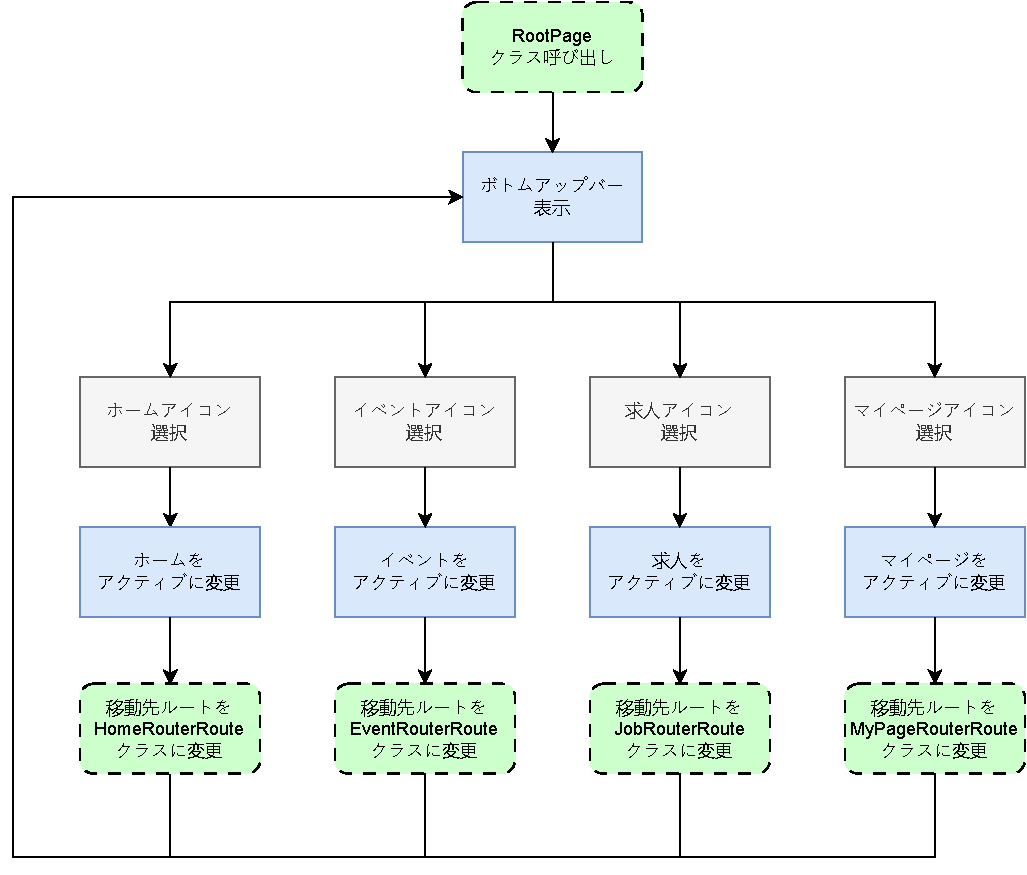
\includegraphics[scale = 1.0]{./images/internal-design/state_change_diagram/root/root_page.pdf}
  \caption{root\_page.dartの状態遷移図}
\end{figure}



\begin{table}[H]
  \centering
  \begin{tabular}{|c|l|l|} \hline
    モジュール名                & \multicolumn{2}{l|}{change\_root\_page.dart}                                                                                              \\ \hline
    モジュール概要               & \multicolumn{2}{p{12cm}|}{アプリ全体を包括するモジュール}                                                                                                \\ \hline
    責任者                   & \multicolumn{2}{l|}{新谷光城}                                                                                                                 \\ \hline
    \multirow{7}{*}{構成要素} & クラス名                                                             & ChangeRootPage                                                         \\ \cline{2-3}
                          & クラス種類                                                            & extends StatelessWidget                                                \\ \cline{2-3}
                          & 処理概要                                                             & \multicolumn{1}{p{12cm}|}{アプリの大まかな区別であるLoginRouteとRootRouteを包括しているクラス} \\ \cline{2-3}
                          & 入力                                                               & なし                                                                     \\ \cline{2-3}
                          & 出力                                                               & Widget                                                                 \\ \cline{2-3}
                          & \multicolumn{2}{l|}{他クラス・関数との関係}                                                                                                          \\ \cline{2-3}
                          & \multicolumn{2}{p{14cm}|}{app\_router.gr.dartのLoginRouteクラスを組み込む
    \newline app\_router.gr.dartのRootRouteクラスを組み込む}                                                                                                                   \\ \hline
  \end{tabular}
\end{table}

\begin{figure}[H]
  \centering
  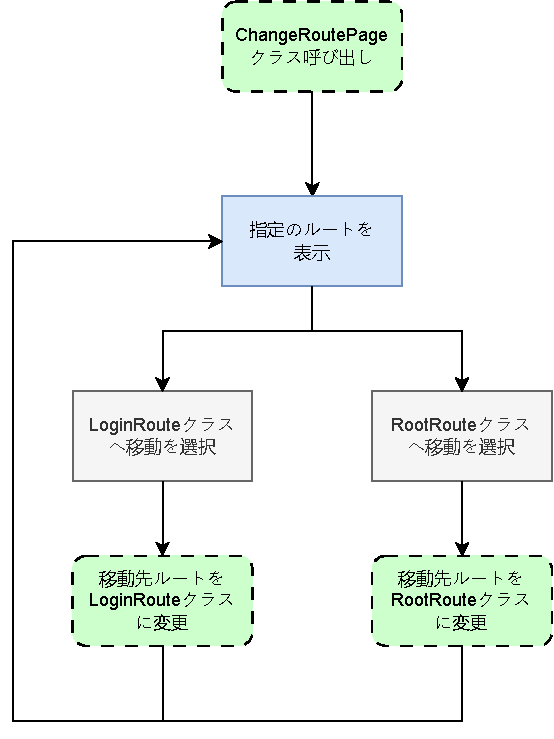
\includegraphics[scale = 1.0]{./images/internal-design/state_change_diagram/root/change_route_page.pdf}
  \caption{change\_root\_page.dartの状態遷移図}
\end{figure}


\clearpage
\begin{longtable}{|c|l|l|}
  \endfirsthead
  \hline
  モジュール名                & \multicolumn{2}{l|}{mypage.dart}                                                                                                                    \\ \hline
  モジュール概要               & \multicolumn{2}{p{12cm}|}{マイページ画面を表示するモジュール}                                                                                                        \\ \hline
  責任者                   & \multicolumn{2}{l|}{新谷光城}                                                                                                                           \\ \hline
  \multirow{7}{*}{構成要素} & クラス名                                                                                         & MyPageRouterPage                                     \\ \cline{2-3}
                        & クラス種類                                                                                        & extends AppRouter                                    \\ \cline{2-3}
                        & 処理概要                                                                                         & \multicolumn{1}{p{12cm}|}{MyPageにアクセスするためのRouter}    \\ \cline{2-3}
                        & 入力                                                                                           & なし                                                   \\ \cline{2-3}
                        & 出力                                                                                           & Route                                                \\ \cline{2-3}
                        & \multicolumn{2}{l|}{他クラス・関数との関係}                                                                                                                    \\ \cline{2-3}
                        & \multicolumn{2}{p{14cm}|}{なし}                                                                                                                       \\ \hline
  \multirow{7}{*}{構成要素} & クラス名                                                                                         & MyPage                                               \\ \cline{2-3}
                        & クラス種類                                                                                        & extends StatelessWidget                              \\ \cline{2-3}
                        & 処理概要                                                                                         & \multicolumn{1}{p{12cm}|}{マイページ画面を動的に変更するクラス}        \\ \cline{2-3}
                        & 入力                                                                                           & なし                                                   \\ \cline{2-3}
                        & 出力                                                                                           & Widget                                               \\ \cline{2-3}
                        & \multicolumn{2}{l|}{他クラス・関数との関係}                                                                                                                    \\ \cline{2-3}
                        & \multicolumn{2}{p{14cm}|}{mypage.dartのMyPageStateクラスを組み込む}                                                                                          \\ \hline
  \multirow{7}{*}{構成要素} & クラス名                                                                                         & MyPageState                                          \\ \cline{2-3}
                        & クラス種類                                                                                        & extends StatelessWidget                              \\ \cline{2-3}
                        & 処理概要                                                                                         & \multicolumn{1}{p{12cm}|}{マイページ画面の状態を返すクラス}          \\ \cline{2-3}
                        & 入力                                                                                           & なし                                                   \\ \cline{2-3}
                        & 出力                                                                                           & State                                                \\ \cline{2-3}
                        & \multicolumn{2}{l|}{他クラス・関数との関係}                                                                                                                    \\ \cline{2-3}
                        & \multicolumn{2}{p{14cm}|}{title\_appbar.dartのTitleAppBarクラスを組み込む
  \newline mypage.dartのScrollMyPageDetailクラスを組み込む}                                                                                                                            \\ \hline
  \multirow{7}{*}{構成要素} & クラス名                                                                                         & ScrollMyPageDetail                                   \\ \cline{2-3}
                        & クラス種類                                                                                        & extends StatelessWidget                              \\ \cline{2-3}
                        & 処理概要                                                                                         & \multicolumn{1}{p{12cm}|}{マイページの画面設定一覧スクロールを作成するクラス} \\ \cline{2-3}
                        & 入力                                                                                           & なし                                                   \\ \cline{2-3}
                        & 出力                                                                                           & Widget                                               \\ \cline{2-3}
                        & \multicolumn{2}{l|}{他クラス・関数との関係}                                                                                                                    \\ \cline{2-3}
                        & \multicolumn{2}{p{14cm}|}{change\_general\_corporation.dartのChangeGeneralCorporationクラスを組み込む
  \newline mypage.dartのMyPageListViewクラスを組み込む}                                                                                                                                \\ \hline
  \multirow{7}{*}{構成要素} & クラス名                                                                                         & MyPageListView                                       \\ \cline{2-3}
                        & クラス種類                                                                                        & extends StatelessWidget                              \\ \cline{2-3}
                        & 処理概要                                                                                         & \multicolumn{1}{p{12cm}|}{設定一覧の小分けを作成するクラス}          \\ \cline{2-3}
                        & 入力                                                                                           & \multicolumn{1}{p{12cm}|}{MediaQueryData data,
    \newline ChangeGeneralCorporation store
    \newline List$<$Map$<$String, dynamic$>$$>$
  \newline String}                                                                                                                                                            \\ \cline{2-3}
                        & 出力                                                                                           & Widget                                               \\ \cline{2-3}
                        & \multicolumn{2}{l|}{他クラス・関数との関係}                                                                                                                    \\ \cline{2-3}
                        & \multicolumn{2}{p{14cm}|}{
    change\_general\_corporation.dartのChangeGeneralCorporationクラスを組み込む
    \newline general\_mem\_inf\_conf.dartのGeneralMemInfConfクラスを呼び出し一般会員情報確認画面を表示
    \newline company\_mem\_inf\_conf.dartのCompanyMemInfConfクラスを呼び出し法人会員情報確認画面を表示
    \newline else\_list.dartのElseListクラスを呼び出しお気に入り登録画面、閲覧履歴画面
    \newline apply\_hist.dartのApplyHistクラスを呼び出し応募履歴画面を表示
    \newline not\_post\_list.dartのNotPostListクラスを呼び出し未振り込み投稿一覧画面を表示
    \newline posted\_list.dartのPostedListクラスを呼び出し投稿広告一覧画面を表示
    \newline event\_fee.dartのEventFeeクラスを呼び出しイベント掲載料金プラン画面を表示
    \newline job\_fee.dartのJobFeeクラスを呼び出し求人掲載料金プラン画面を表示
    \newline transfer\_to.dartのTransferToクラスを呼び出し振込先口座番号表示画面を表示
    \newline ask\_page.dartのAskPageクラスを呼び出し問い合わせ画面表示
    \newline rule\_screen.dartのRuleScreenクラスを呼び出し利用規約オーバーレイを表示
    \newline log\_out.dartのLogOutクラスを呼び出しログアウトオーバーレイを表示
    \newline secession.dartのSecessionクラスを呼び出し退会オーバーレイを表示
  }                                                                                                                                                                           \\ \hline
\end{longtable}


\begin{figure}[H]
  \centering
  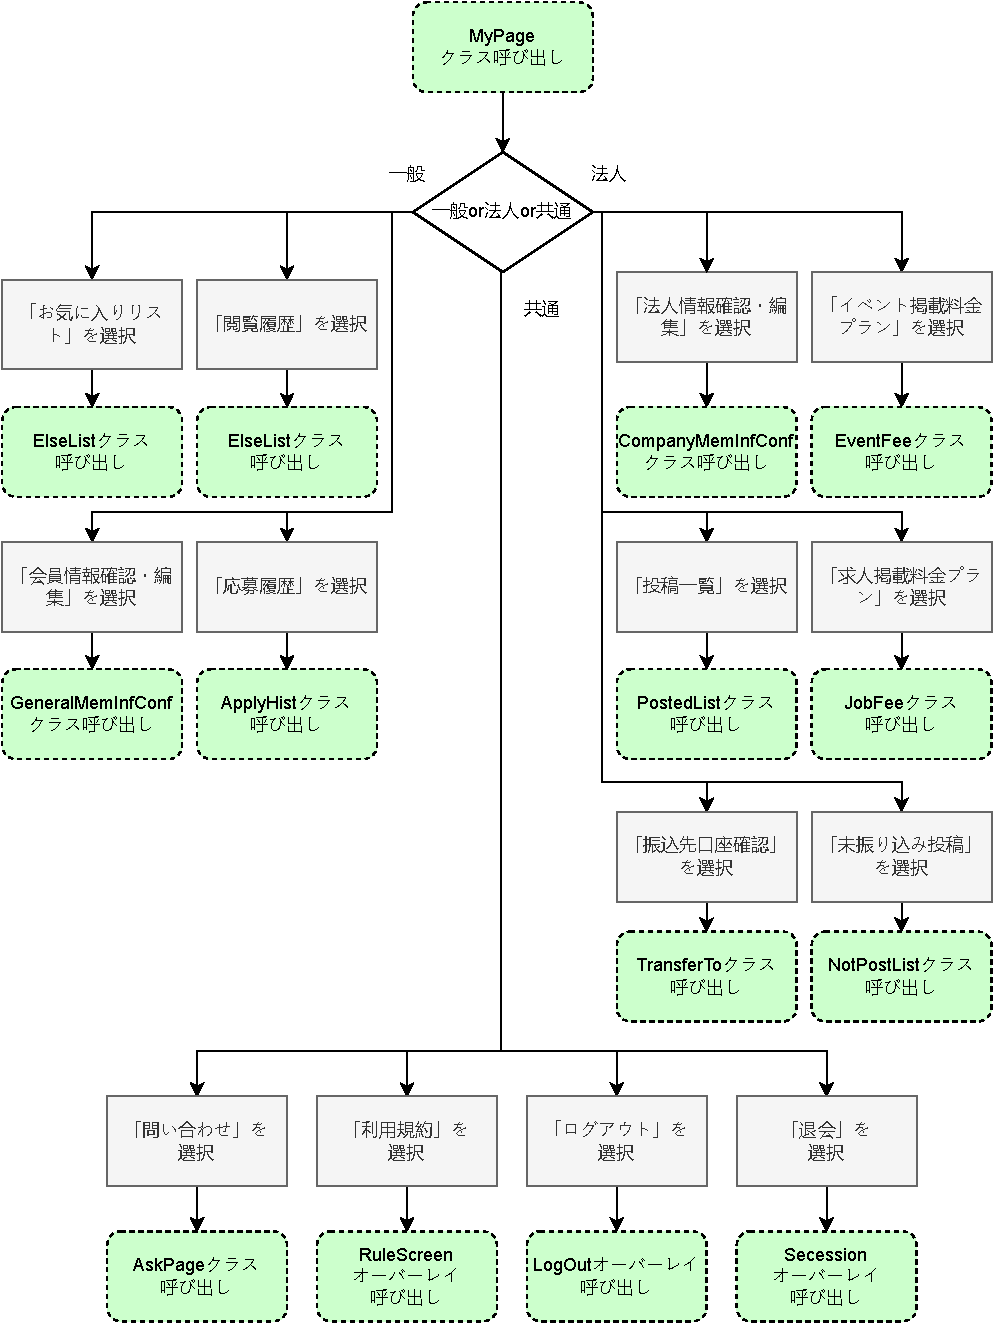
\includegraphics[width=15cm]{./images/internal-design/state_change_diagram/mypage/mypage.pdf}
  \caption{mypage.dartの状態遷移図}
\end{figure}

% \begin{table}[H]
%   \centering
%   \begin{tabular}{|c|l|l|} \hline

%   \end{tabular}
% \end{table}

\begin{table}[H]
  \centering
  \begin{tabular}{|c|l|l|} \hline
    モジュール名                & \multicolumn{2}{l|}{general\_mem\_inf\_conf.dart}                                                                                    \\ \hline
    モジュール概要               & \multicolumn{2}{p{12cm}|}{一般会員情報確認画面を表示するモジュール}                                                                                      \\ \hline
    責任者                   & \multicolumn{2}{l|}{新谷光城}                                                                                                            \\ \hline
    \multirow{7}{*}{構成要素} & クラス名                                                                              & GeneralMemInfConf                                \\ \cline{2-3}
                          & クラス種類                                                                             & extends StatelessWidget                          \\ \cline{2-3}
                          & 処理概要                                                                              & \multicolumn{1}{p{12cm}|}{一般会員情報確認画面を動的に変更するクラス} \\ \cline{2-3}
                          & 入力                                                                                & なし                                               \\ \cline{2-3}
                          & 出力                                                                                & Widget                                           \\ \cline{2-3}
                          & \multicolumn{2}{l|}{他クラス・関数との関係}                                                                                                     \\ \cline{2-3}
                          & \multicolumn{2}{p{14cm}|}{general\_mem\_inf\_conf.dartのGeneralMemInfConfクラスを組み込み}                                                    \\ \hline
    \multirow{7}{*}{構成要素} & クラス名                                                                              & GeneralMemInfConfState                           \\ \cline{2-3}
                          & クラス種類                                                                             & extends StatelessWidget                          \\ \cline{2-3}
                          & 処理概要                                                                              & \multicolumn{1}{p{12cm}|}{一般会員情報確認画面の状態を返すクラス}   \\ \cline{2-3}
                          & 入力                                                                                & なし                                               \\ \cline{2-3}
                          & 出力                                                                                & State                                            \\ \cline{2-3}
                          & \multicolumn{2}{l|}{他クラス・関数との関係}                                                                                                     \\ \cline{2-3}
                          & \multicolumn{2}{p{14cm}|}{
      change\_generalcorporation.dartのChangeGeneralCorporationプロバイダを組み込む
      \newline title\_appbar.dartのTitleAppBarクラスを組み込む
      \newline general\_mem\_inf\_change.dartのGeneralMemInfChangeクラスを呼び出し一般会員情報変更画面を表示
      \newline pass\_change.dartのPassChangeクラスを呼び出しパスワード変更画面を表示
    \newline 戻るボタンの選択で前のモジュールに戻る}                                                                                                                                \\ \hline
  \end{tabular}
\end{table}

\begin{figure}[H]
  \centering
  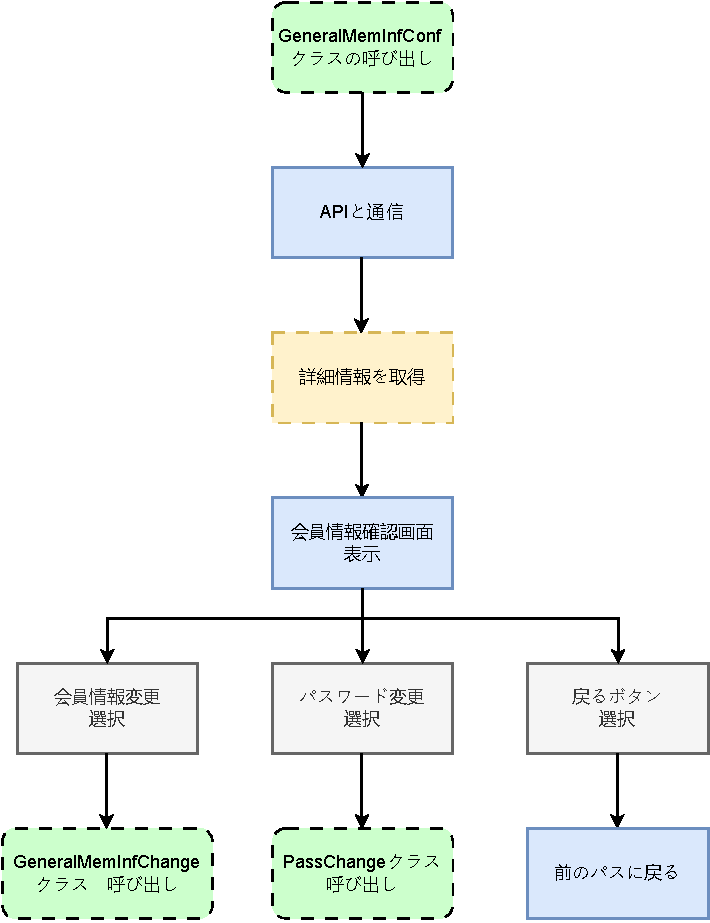
\includegraphics[width=15cm]{./images/internal-design/state_change_diagram/mypage/general_mem_inf_conf.pdf}
  \caption{general\_mem\_inf\_conf.dartの状態遷移図}
\end{figure}

\begin{table}[H]
  \centering
  \begin{tabular}{|c|l|l|} \hline
    モジュール名                & \multicolumn{2}{l|}{general\_mem\_inf\_change.dart}                                                                                           \\ \hline
    モジュール概要               & \multicolumn{2}{p{12cm}|}{一般会員情報変更画面を表示するモジュール}                                                                                               \\ \hline
    責任者                   & \multicolumn{2}{l|}{新谷光城}                                                                                                                     \\ \hline
    \multirow{7}{*}{構成要素} & クラス名                                                                                       & GeneralMemInfChange                              \\ \cline{2-3}
                          & クラス種類                                                                                      & extends StatelessWidget                          \\ \cline{2-3}
                          & 処理概要                                                                                       & \multicolumn{1}{p{12cm}|}{一般会員情報変更画面を動的に変更するクラス} \\ \cline{2-3}
                          & 入力                                                                                         & なし                                               \\ \cline{2-3}
                          & 出力                                                                                         & Widget                                           \\ \cline{2-3}
                          & \multicolumn{2}{l|}{他クラス・関数との関係}                                                                                                              \\ \cline{2-3}
                          & \multicolumn{2}{p{14cm}|}{general\_mem\_inf\_change.dartのGeneralMemInfChangeStateクラスを組み込み}                                                    \\ \hline
    \multirow{7}{*}{構成要素} & クラス名                                                                                       & GeneralMemInfChangeState                         \\ \cline{2-3}
                          & クラス種類                                                                                      & extends StatelessWidget                          \\ \cline{2-3}
                          & 処理概要                                                                                       & \multicolumn{1}{p{12cm}|}{一般会員情報変更画面の状態を返すクラス}   \\ \cline{2-3}
                          & 入力                                                                                         & なし                                               \\ \cline{2-3}
                          & 出力                                                                                         & State                                            \\ \cline{2-3}
                          & \multicolumn{2}{l|}{他クラス・関数との関係}                                                                                                              \\ \cline{2-3}
                          & \multicolumn{2}{p{14cm}|}{
      change\_generalcorporation.dartのChangeGeneralCorporationプロバイダを組み込む
      \newline title\_appbar.dartのTitleAppBarクラスを組み込む
      \newline general\_mem\_inf\_conf.dartのGeneralMemInfConfクラスを呼び出し一般会員情報確認画面を表示
    \newline 戻るボタンの選択で前のモジュールに戻る}                                                                                                                                         \\ \hline
  \end{tabular}
\end{table}

\begin{figure}[H]
  \centering
  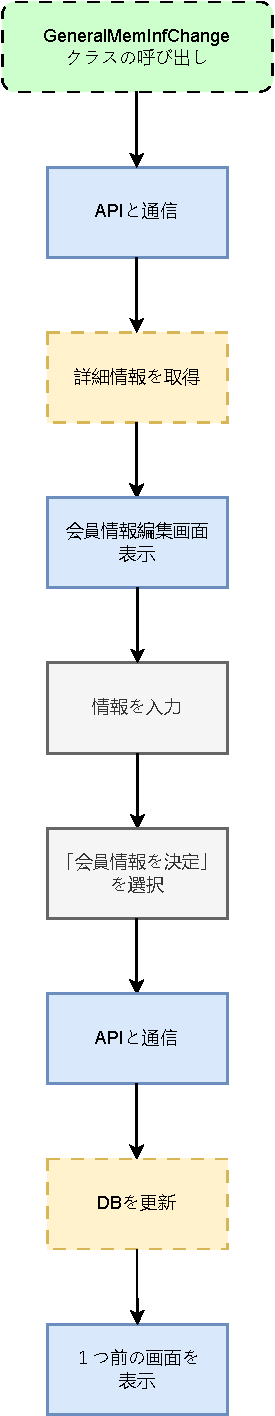
\includegraphics[width=4.5cm]{./images/internal-design/state_change_diagram/mypage/general_mem_inf_change.pdf}
  \caption{general\_mem\_inf\_change.dartの状態遷移図}
\end{figure}

\begin{table}[H]
  \centering
  \begin{tabular}{|c|l|l|} \hline
    モジュール名                & \multicolumn{2}{l|}{apply\_conf.dart}                                                                           \\ \hline
    モジュール概要               & \multicolumn{2}{p{12cm}|}{投稿した求人に応募を行ったユーザの情報を確認する画面を表示するモジュール}                                                 \\ \hline
    責任者                   & \multicolumn{2}{l|}{新谷光城}                                                                                       \\ \hline
    \multirow{7}{*}{構成要素} & クラス名                                                            & ApplyConf                                     \\ \cline{2-3}
                          & クラス種類                                                           & extends StatelessWidget                       \\ \cline{2-3}
                          & 処理概要                                                            & \multicolumn{1}{p{12cm}|}{応募者確認画面を動的に変更するクラス} \\ \cline{2-3}
                          & 入力                                                              & List$<$Map$<$String, dynamic$>$$>$ profiles   \\ \cline{2-3}
                          & 出力                                                              & Widget                                        \\ \cline{2-3}
                          & \multicolumn{2}{l|}{他クラス・関数との関係}                                                                                \\ \cline{2-3}
                          & \multicolumn{2}{p{14cm}|}{ApplyConfStateを組み込む}                                                                  \\ \hline
    \multirow{7}{*}{構成要素} & クラス名                                                            & ApplyConfState                                \\ \cline{2-3}
                          & クラス種類                                                           & extends StatelessWidget                       \\ \cline{2-3}
                          & 処理概要                                                            & \multicolumn{1}{p{12cm}|}{応募者確認画面の状態を返すクラス}   \\ \cline{2-3}
                          & 入力                                                              & なし                                            \\ \cline{2-3}
                          & 出力                                                              & State                                         \\ \cline{2-3}
                          & \multicolumn{2}{l|}{他クラス・関数との関係}                                                                                \\ \cline{2-3}
                          & \multicolumn{2}{p{14cm}|}{
      ApplyConfStateを組み込む
      \newline conf\_conf.dartのConfConfクラスを呼び出し確認確認オーバーレイを表示
    \newline 戻るボタンの選択で前のモジュールに戻る}                                                                                                           \\ \hline
  \end{tabular}
\end{table}

\begin{figure}[H]
  \centering
  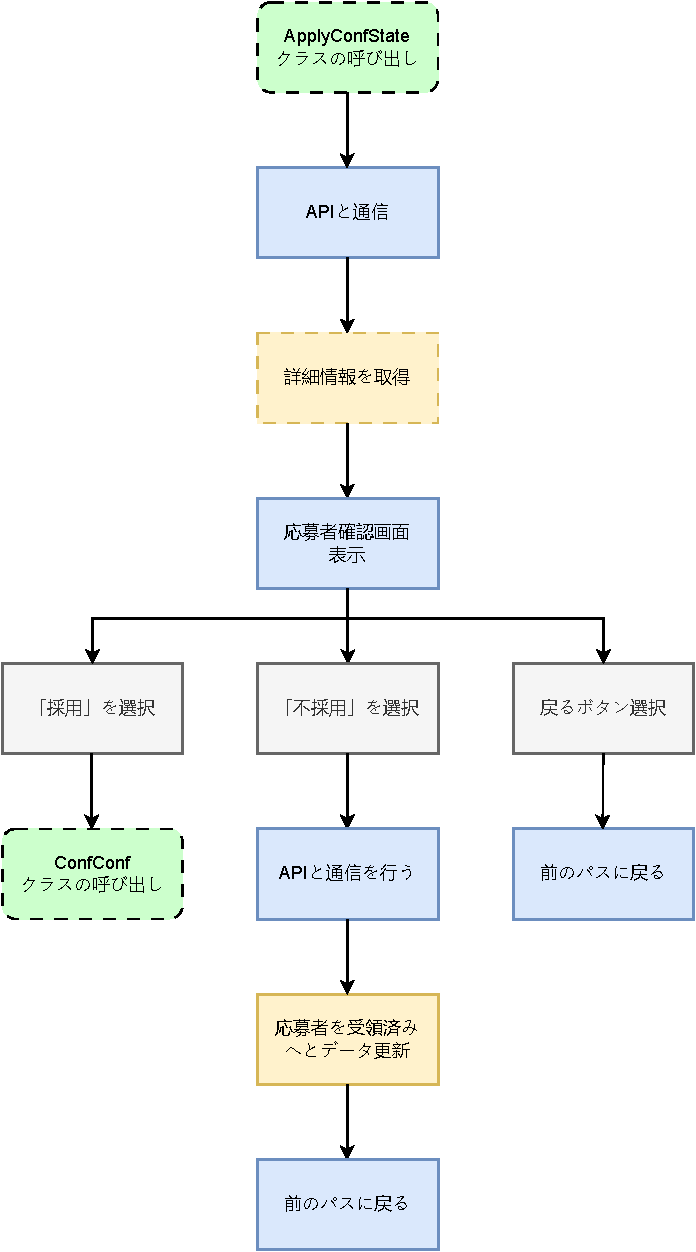
\includegraphics[width=14cm]{./images/internal-design/state_change_diagram/mypage/apply_conf.pdf}
  \caption{apply\_conf.dartの状態遷移図}
\end{figure}

\begin{table}[H]
  \centering
  \begin{tabular}{|c|l|l|} \hline
    モジュール名                & \multicolumn{2}{l|}{transfer\_to.dart}                                                        \\ \hline
    モジュール概要               & \multicolumn{2}{p{12cm}|}{振込先口座表示画面を表示するモジュール}                                                \\ \hline
    責任者                   & \multicolumn{2}{l|}{新谷光城}                                                                     \\ \hline
    \multirow{7}{*}{構成要素} & クラス名                                           & TransferTo                                   \\ \cline{2-3}
                          & クラス種類                                          & extends StatelessWidget                      \\ \cline{2-3}
                          & 処理概要                                           & \multicolumn{1}{p{12cm}|}{振込先口座表示番号を表示するクラス} \\ \cline{2-3}
                          & 入力                                             & なし                                           \\ \cline{2-3}
                          & 出力                                             & Widget                                       \\ \cline{2-3}
                          & \multicolumn{2}{l|}{他クラス・関数との関係}                                                              \\ \cline{2-3}
                          & \multicolumn{2}{p{14cm}|}{戻るボタンの選択で前のモジュールに戻る}                                                \\ \hline
  \end{tabular}
\end{table}

\begin{figure}[H]
  \centering
  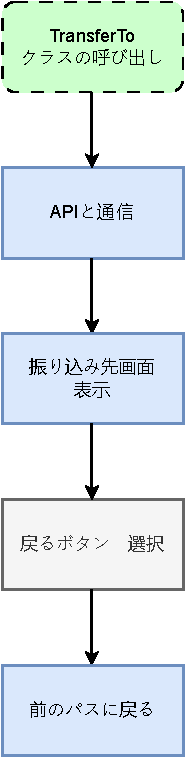
\includegraphics[width=4.5cm]{./images/internal-design/state_change_diagram/mypage/transfer_to.pdf}
  \caption{transfer\_to.dartの状態遷移図}
\end{figure}


\begin{table}[H]
  \centering
  \begin{tabular}{|c|l|l|} \hline
    モジュール名                & \multicolumn{2}{l|}{company\_mem\_inf\_conf.dart}                                                                                    \\ \hline
    モジュール概要               & \multicolumn{2}{p{12cm}|}{法人会員情報確認画面を表示するモジュール}                                                                                      \\ \hline
    責任者                   & \multicolumn{2}{l|}{新谷光城}                                                                                                            \\ \hline
    \multirow{7}{*}{構成要素} & クラス名                                                                              & CompanyMemInfConf                                \\ \cline{2-3}
                          & クラス種類                                                                             & extends StatelessWidget                          \\ \cline{2-3}
                          & 処理概要                                                                              & \multicolumn{1}{p{12cm}|}{法人会員情報確認画面を動的に変更するクラス} \\ \cline{2-3}
                          & 入力                                                                                & なし                                               \\ \cline{2-3}
                          & 出力                                                                                & Widget                                           \\ \cline{2-3}
                          & \multicolumn{2}{l|}{他クラス・関数との関係}                                                                                                     \\ \cline{2-3}
                          & \multicolumn{2}{p{14cm}|}{company\_mem\_inf\_conf.dartのGeneralMemInfConfクラスを組み込み}                                                    \\ \hline
    \multirow{7}{*}{構成要素} & クラス名                                                                              & CompanyMemInfConfState                           \\ \cline{2-3}
                          & クラス種類                                                                             & extends StatelessWidget                          \\ \cline{2-3}
                          & 処理概要                                                                              & \multicolumn{1}{p{12cm}|}{法人会員情報確認画面の状態を返すクラス}   \\ \cline{2-3}
                          & 入力                                                                                & なし                                               \\ \cline{2-3}
                          & 出力                                                                                & State                                            \\ \cline{2-3}
                          & \multicolumn{2}{l|}{他クラス・関数との関係}                                                                                                     \\ \cline{2-3}
                          & \multicolumn{2}{p{14cm}|}{
      change\_generalcorporation.dartのChangeGeneralCorporationプロバイダを組み込む
      \newline title\_appbar.dartのTitleAppBarクラスを組み込む
      \newline cmopany\_mem\_inf\_change.dartのCompanyMemInfChangeクラスを呼び出し法人会員情報変更画面を表示
      \newline pass\_change.dartのPassChangeクラスを呼び出しパスワード変更画面を表示
    \newline 戻るボタンの選択で前のモジュールに戻る}                                                                                                                                \\ \hline
  \end{tabular}
\end{table}

\begin{figure}[H]
  \centering
  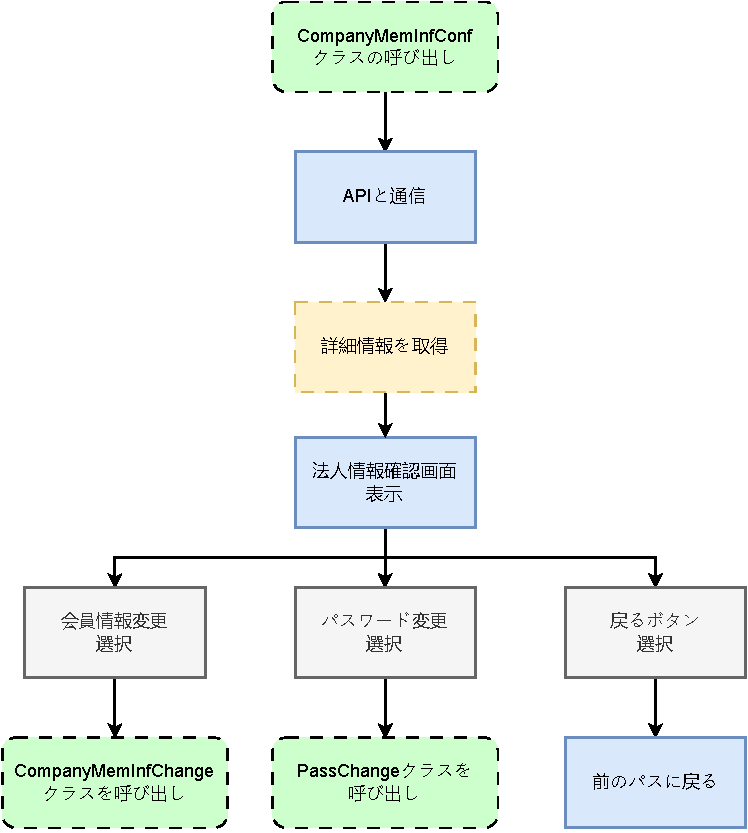
\includegraphics[width=17cm]{./images/internal-design/state_change_diagram/mypage/company_mem_inf_conf.pdf}
  \caption{company\_mem\_inf\_conf.dartの状態遷移図}
\end{figure}


\begin{table}[H]
  \centering
  \begin{tabular}{|c|l|l|} \hline
    モジュール名                & \multicolumn{2}{l|}{company\_mem\_inf\_change.dart}                                                                                      \\ \hline
    モジュール概要               & \multicolumn{2}{p{12cm}|}{法人会員情報編集画面を表示するモジュール}                                                                                          \\ \hline
    責任者                   & \multicolumn{2}{l|}{山本昇永}                                                                                                                \\ \hline
    \multirow{7}{*}{構成要素} & クラス名                                                                                  & CompanyMemInfChange                              \\ \cline{2-3}
                          & クラス種類                                                                                 & extends StatelessWidget                          \\ \cline{2-3}
                          & 処理概要                                                                                  & \multicolumn{1}{p{12cm}|}{法人会員情報編集画面を動的に変更するクラス} \\ \cline{2-3}
                          & 入力                                                                                    & なし                                               \\ \cline{2-3}
                          & 出力                                                                                    & Widget                                           \\ \cline{2-3}
                          & \multicolumn{2}{l|}{他クラス・関数との関係}                                                                                                         \\ \cline{2-3}
                          & \multicolumn{2}{p{14cm}|}{company\_mem\_inf\_change.dartのGeneralMemInfChangeクラスを組み込み}                                                    \\ \hline
    \multirow{7}{*}{構成要素} & クラス名                                                                                  & CompanyMemInfChangeState                         \\ \cline{2-3}
                          & クラス種類                                                                                 & extends StatelessWidget                          \\ \cline{2-3}
                          & 処理概要                                                                                  & \multicolumn{1}{p{12cm}|}{法人会員情報編集画面の状態を返すクラス}   \\ \cline{2-3}
                          & 入力                                                                                    & なし                                               \\ \cline{2-3}
                          & 出力                                                                                    & State                                            \\ \cline{2-3}
                          & \multicolumn{2}{l|}{他クラス・関数との関係}                                                                                                         \\ \cline{2-3}
                          & \multicolumn{2}{p{14cm}|}{
      change\_generalcorporation.dartのChangeGeneralCorporationプロバイダを組み込む
      \newline title\_appbar.dartのTitleAppBarクラスを組み込む
      \newline company\_form.dartのCompanyFormクラスを組み込む
    \newline 戻るボタンの選択で前のモジュールに戻る}                                                                                                                                    \\ \hline
  \end{tabular}
\end{table}

\begin{figure}[H]
  \centering
  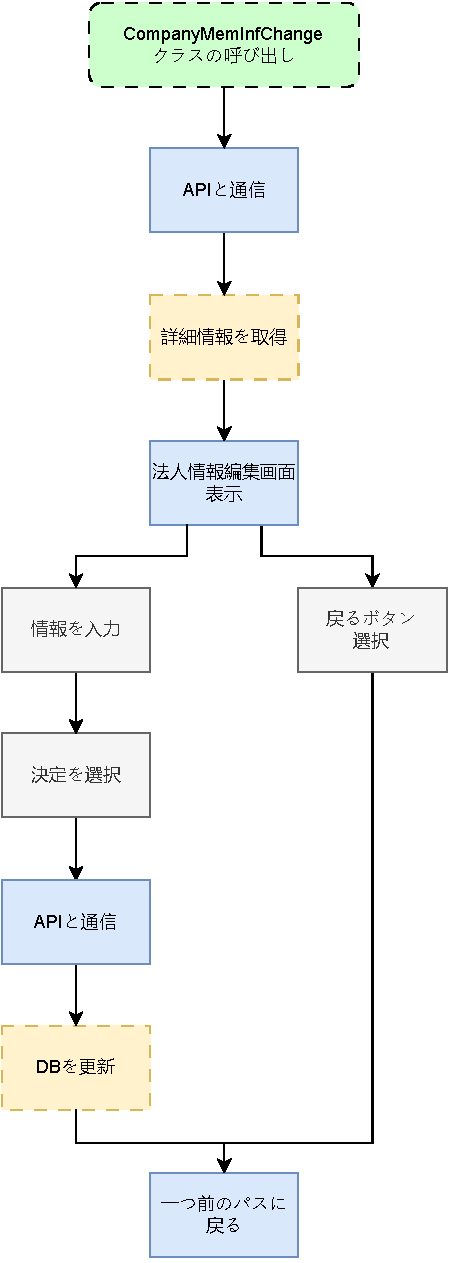
\includegraphics[width=9cm]{./images/internal-design/state_change_diagram/mypage/company_mem_inf_change.pdf}
  \caption{company\_mem\_inf\_change.dartの状態遷移図}
\end{figure}

\begin{table}[H]
  \centering
  \begin{tabular}{|c|l|l|} \hline
    モジュール名                & \multicolumn{2}{l|}{event\_fee.dart}                                                                   \\ \hline
    モジュール概要               & \multicolumn{2}{p{12cm}|}{イベント広告の掲載料金プランを表示するモジュール}                                                    \\ \hline
    責任者                   & \multicolumn{2}{l|}{新谷光城}                                                                              \\ \hline
    \multirow{7}{*}{構成要素} & クラス名                                                & EventFee                                         \\ \cline{2-3}
                          & クラス種類                                               & extends StatelessWidget                          \\ \cline{2-3}
                          & 処理概要                                                & \multicolumn{1}{p{12cm}|}{イベント広告掲載料金プランを表示するクラス} \\ \cline{2-3}
                          & 入力                                                  & なし                                               \\ \cline{2-3}
                          & 出力                                                  & Widget                                           \\ \cline{2-3}
                          & \multicolumn{2}{l|}{他クラス・関数との関係}                                                                       \\ \cline{2-3}
                          & \multicolumn{2}{p{14cm}|}{
      change\_generalcorporation.dartのChangeGeneralCorporationプロバイダを組み込む
      \newline event\_fee\_select.dartのEventPostInfoプロバイダを組み込む
      \newline title\_appbar.dartのTitleAppBarクラスを組み込む
      \newline transfer\_to.dartのTransferToクラスを呼び出し振込口座確認画面を表示
      \newline 戻るボタンの選択で前のモジュールに戻る
    }                                                                                                                              \\ \hline
  \end{tabular}
\end{table}

\begin{figure}[H]
  \centering
  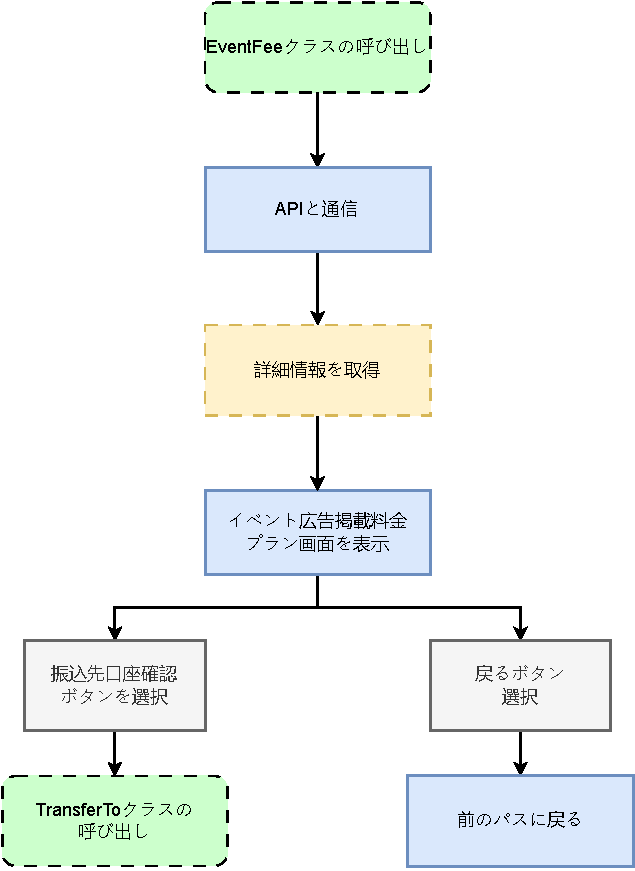
\includegraphics[width=12cm]{./images/internal-design/state_change_diagram/mypage/event_fee.pdf}
  \caption{event\_fee.dartの状態遷移図}
\end{figure}



\begin{table}[H]
  \centering
  \begin{tabular}{|c|l|l|} \hline
    モジュール名                & \multicolumn{2}{l|}{event\_fee\_select.dart}                                                                \\ \hline
    モジュール概要               & \multicolumn{2}{p{12cm}|}{イベント掲載料金プランを選択する画面を表示するモジュール}                                                     \\ \hline
    責任者                   & \multicolumn{2}{l|}{新谷光城}                                                                                   \\ \hline
    \multirow{7}{*}{構成要素} & クラス名                                                    & EventFeeSelect                                    \\ \cline{2-3}
                          & クラス種類                                                   & extends StatelessWidget                           \\ \cline{2-3}
                          & 処理概要                                                    & \multicolumn{1}{p{12cm}|}{求人掲載料金プラン選択画面を表示するクラス}  \\ \cline{2-3}
                          & 入力                                                      & なし                                                \\ \cline{2-3}
                          & 出力                                                      & Widget                                            \\ \cline{2-3}
                          & \multicolumn{2}{l|}{他クラス・関数との関係}                                                                            \\ \cline{2-3}
                          & \multicolumn{2}{p{14cm}|}{
      change\_generalcorporation.dartのChangeGeneralCorporationプロバイダを組み込む
      \newline event\_fee\_select.dartのEventPostInfoプロバイダを組み込む
      \newline title\_appbar.dartのTitleAppBarクラスを組み込む
      \newline job\_post\_write.dartのJobPostWriteクラスを呼び出し求人広告掲載内容記述画面を表示
    \newline 戻るボタンの選択で前のモジュールに戻る}                                                                                                       \\ \hline
    \multirow{7}{*}{構成要素} & クラス名                                                    & EventPostInfo                                     \\ \cline{2-3}
                          & クラス種類                                                   & ChangeNotifier                                    \\ \cline{2-3}
                          & 処理概要                                                    & \multicolumn{1}{p{12cm}|}{イベント広告投稿内容を保存しておくプロバイダ} \\ \cline{2-3}
                          & 入力                                                      & なし                                                \\ \cline{2-3}
                          & 出力                                                      & なし                                                \\ \cline{2-3}
                          & \multicolumn{2}{l|}{他クラス・関数との関係}                                                                            \\ \cline{2-3}
                          & \multicolumn{2}{p{14cm}|}{なし}                                                                               \\ \hline
  \end{tabular}
\end{table}

\begin{figure}[H]
  \centering
  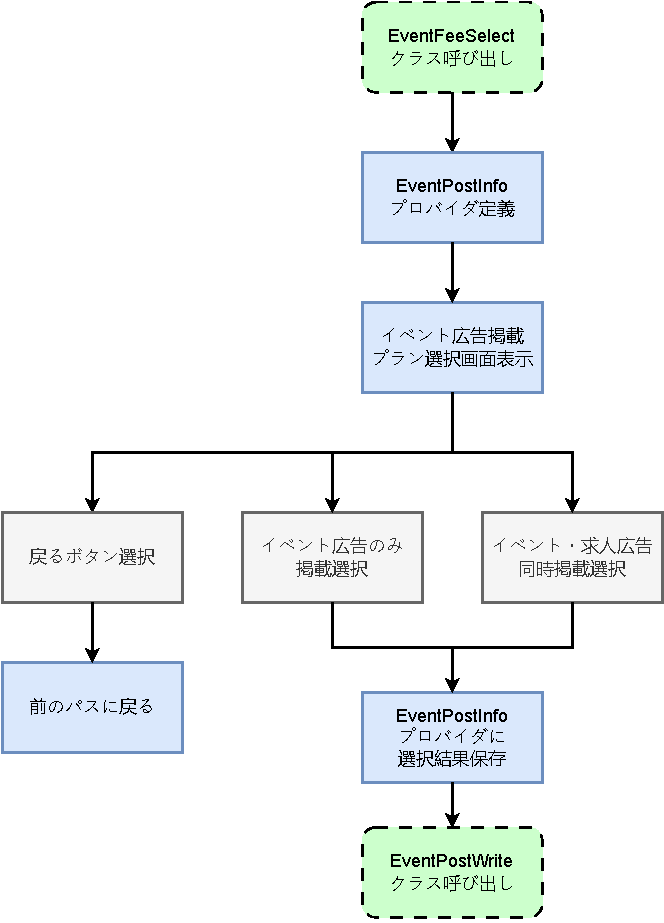
\includegraphics[width=15cm]{./images/internal-design/state_change_diagram/mypage/event_fee_select.pdf}
  \caption{event\_fee\_select.dartの状態遷移図}
\end{figure}

\begin{table}[H]
  \centering
  \begin{tabular}{|c|l|l|} \hline
    モジュール名                & \multicolumn{2}{l|}{job\_fee.dart}                                                                \\ \hline
    モジュール概要               & \multicolumn{2}{p{12cm}|}{求人広告の掲載料金プランを表示するレイヤー}                                                  \\ \hline
    責任者                   & \multicolumn{2}{l|}{新谷光城}                                                                         \\ \hline
    \multirow{7}{*}{構成要素} & クラス名                                             & JobFee                                         \\ \cline{2-3}
                          & クラス種類                                            & extends StatelessWidget                        \\ \cline{2-3}
                          & 処理概要                                             & \multicolumn{1}{p{12cm}|}{求人広告掲載料金プランを表示するクラス} \\ \cline{2-3}
                          & 入力                                               & 契約希望月(int)                                     \\ \cline{2-3}
                          & 出力                                               & Widget                                         \\ \cline{2-3}
                          & \multicolumn{2}{l|}{他クラス・関数との関係}                                                                  \\ \cline{2-3}
                          & \multicolumn{2}{p{14cm}|}{
      change\_generalcorporation.dartのChangeGeneralCorporationプロバイダを組み込む
      \newline job\_fee\_select.dartのJobPostInfoプロバイダを組み込む
      \newline title\_appbar.dartのTitleAppBarクラスを組み込む
      \newline transfer\_to.dartのTransferToクラスを呼び出し振込口座確認画面を表示
      \newline 戻るボタンの選択で前のモジュールに戻る
    }                                                                                                                         \\ \hline
  \end{tabular}
\end{table}

\begin{figure}[H]
  \centering
  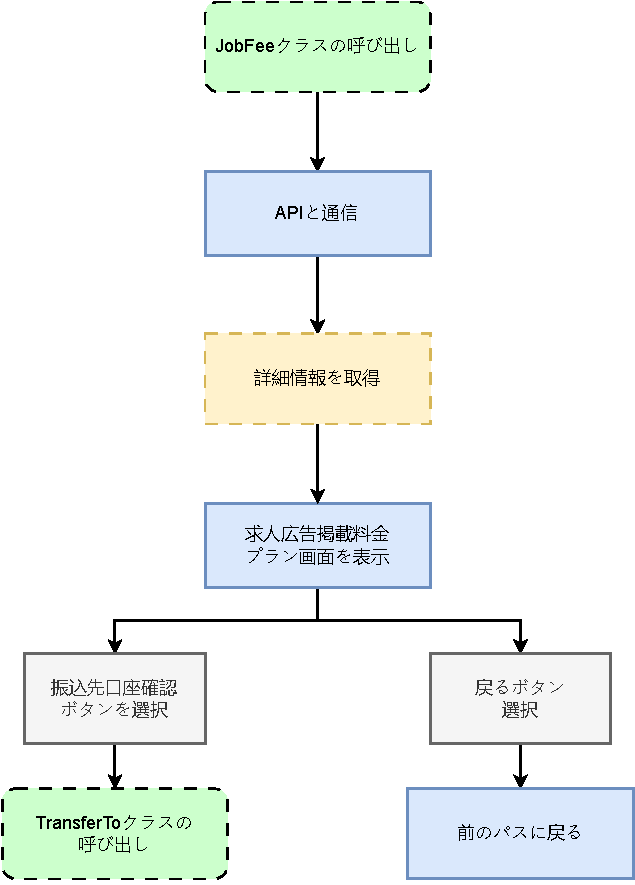
\includegraphics[width=11cm]{./images/internal-design/state_change_diagram/mypage/job_fee.pdf}
  \caption{job\_fee.dartの状態遷移図}
\end{figure}




\begin{table}[H]
  \centering
  \begin{tabular}{|c|l|l|} \hline
    モジュール名                & \multicolumn{2}{l|}{job\_fee\_select.dart}                                                               \\ \hline
    モジュール概要               & \multicolumn{2}{p{12cm}|}{求人掲載料金プランを選択する画面を表示するモジュール}                                                    \\ \hline
    責任者                   & \multicolumn{2}{l|}{新谷光城}                                                                                \\ \hline
    \multirow{7}{*}{構成要素} & クラス名                                                  & JobFeeSelect                                     \\ \cline{2-3}
                          & クラス種類                                                 & extends StatelessWidget                          \\ \cline{2-3}
                          & 処理概要                                                  & \multicolumn{1}{p{12cm}|}{求人掲載料金プラン選択画面を表示するクラス} \\ \cline{2-3}
                          & 入力                                                    & なし                                               \\ \cline{2-3}
                          & 出力                                                    & Widget                                           \\ \cline{2-3}
                          & \multicolumn{2}{l|}{他クラス・関数との関係}                                                                         \\ \cline{2-3}
                          & \multicolumn{2}{p{14cm}|}{
      change\_generalcorporation.dartのChangeGeneralCorporationプロバイダを組み込む
      \newline job\_fee\_select.dartのJobPostInfoプロバイダを組み込む
      \newline title\_appbar.dartのTitleAppBarクラスを組み込む
      \newline transfer\_to.dartのTransferToクラスを呼び出し振込口座確認画面を表示
      \newline event\_post\_write.dartのEventPostWriteクラスを呼び出しイベント広告掲載内容記述画面を表示
    \newline 戻るボタンの選択で前のモジュールに戻る}                                                                                                    \\ \hline
    \multirow{7}{*}{構成要素} & クラス名                                                  & JobPostInfo                                      \\ \cline{2-3}
                          & クラス種類                                                 & ChangeNotifier                                   \\ \cline{2-3}
                          & 処理概要                                                  & \multicolumn{1}{p{12cm}|}{求人広告投稿内容を保存しておくプロバイダ}  \\ \cline{2-3}
                          & 入力                                                    & なし                                               \\ \cline{2-3}
                          & 出力                                                    & なし                                               \\ \cline{2-3}
                          & \multicolumn{2}{l|}{他クラス・関数との関係}                                                                         \\ \cline{2-3}
                          & \multicolumn{2}{p{14cm}|}{なし}                                                                            \\ \hline
  \end{tabular}
\end{table}

\begin{figure}[H]
  \centering
  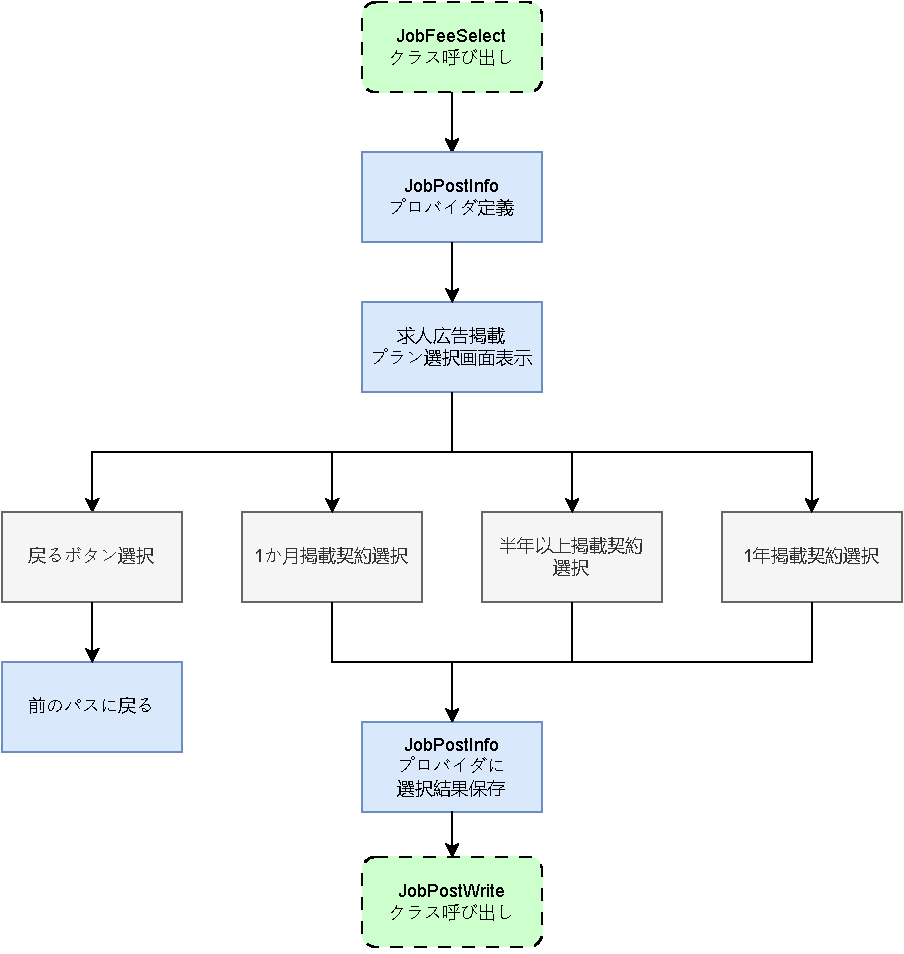
\includegraphics[width=17cm]{./images/internal-design/state_change_diagram/mypage/job_fee_select.pdf}
  \caption{job\_fee\_select.dartの状態遷移図}
\end{figure}


% \begin{table}[H]
%   \centering
%   \begin{tabular}{|c|l|l|} \hline
%     モジュール名                & \multicolumn{2}{l|}{post\_write\_comp.dart}                                                                            \\ \hline
%     モジュール概要               & \multicolumn{2}{p{12cm}|}{投稿したいと考えている内容が投稿時どのように見えるのかの確認を行う画面を表示するモジュール}                                               \\ \hline
%     責任者                   & \multicolumn{2}{l|}{新谷光城}                                                                                              \\ \hline
%     \multirow{7}{*}{構成要素} & クラス名                                                                     & PostWriteComp                               \\ \cline{2-3}
%                           & クラス種類                                                                    & extends StatelessWidget                     \\ \cline{2-3}
%                           & 処理概要                                                                     & \multicolumn{1}{p{12cm}|}{投稿内容確認画面を表示するクラス} \\ \cline{2-3}
%                           & 入力                                                                       & なし                                          \\ \cline{2-3}
%                           & 出力                                                                       & Widget                                      \\ \cline{2-3}
%                           & \multicolumn{2}{l|}{他クラス・関数との関係}                                                                                       \\ \cline{2-3}
%                           & \multicolumn{2}{p{14cm}|}{
%       change\_generalcorporation.dartのChangeGeneralCorporationプロバイダを組み込む
%       \newline job\_fee\_select.dartのJobPostInfoプロバイダを組み込む
%       \newline event\_fee\_select.dartのEventPostInfoプロバイダを組み込む
%       \newline title\_appbar.dartのTitleAppBarクラスを組み込む
%       \newline post\_conf.dartのPostConfクラスを呼び出し投稿確認オーバーレイを表示
%       \newline return\_write.dartのReturnWriteクラスを呼び出し必須内容記入漏れ注意オーバーレイを表示
%       \newline move\_conf.dartのMoveConfクラスを呼び出し投稿中に移動確認オーバーレイを表示
%     \newline 戻るボタンの選択で前のモジュールに戻る}                                                                                                                  \\ \hline
%   \end{tabular}
% \end{table}

% \begin{table}[H]
%   \centering
%   \begin{tabular}{|c|l|l|} \hline
%     モジュール名                & \multicolumn{2}{l|}{job\_post\_write.dart}                                                        \\ \hline
%     モジュール概要               & \multicolumn{2}{p{12cm}|}{イベント広告内容記述画面を表示するモジュール}                                                 \\ \hline
%     責任者                   & \multicolumn{2}{l|}{新谷光城}                                                                         \\ \hline
%     \multirow{7}{*}{構成要素} & クラス名                                              & JobPostWrite                                  \\ \cline{2-3}
%                           & クラス種類                                             & extends StatelessWidget                       \\ \cline{2-3}
%                           & 処理概要                                              & \multicolumn{1}{p{12cm}|}{求人広告内容記述画面を表示するクラス} \\ \cline{2-3}
%                           & 入力                                                & なし                                            \\ \cline{2-3}
%                           & 出力                                                & Widget                                        \\ \cline{2-3}
%                           & \multicolumn{2}{l|}{他クラス・関数との関係}                                                                  \\ \cline{2-3}
%                           & \multicolumn{2}{p{14cm}|}{
%       change\_generalcorporation.dartのChangeGeneralCorporationプロバイダを組み込む
%       \newline job\_fee\_select.dartのJobPostInfoプロバイダを組み込む
%       \newline title\_appbar.dartのTitleAppBarクラスを組み込む
%       \newline post\_conf.dartのPostConfクラスを呼び出し投稿確認オーバーレイを表示
%       \newline return\_write.dartのReturnWriteクラスを呼び出し必須内容記入漏れ注意オーバーレイを表示
%       \newline move\_conf.dartのMoveConfクラスを呼び出し投稿中に移動確認オーバーレイを表示
%     \newline 戻るボタンの選択で前のモジュールに戻る}                                                                                             \\ \hline
%   \end{tabular}
% \end{table}

% \begin{table}[H]
%   \centering
%   \begin{tabular}{|c|l|l|} \hline
%     モジュール名                & \multicolumn{2}{l|}{event\_post\_write.dart}                                                        \\ \hline
%     モジュール概要               & \multicolumn{2}{p{12cm}|}{イベント広告内容記述画面を表示するモジュール}                                                   \\ \hline
%     責任者                   & \multicolumn{2}{l|}{新谷光城}                                                                           \\ \hline
%     \multirow{7}{*}{構成要素} & クラス名                                              & EventPostWrite                                  \\ \cline{2-3}
%                           & クラス種類                                             & extends StatelessWidget                         \\ \cline{2-3}
%                           & 処理概要                                              & \multicolumn{1}{p{12cm}|}{イベント広告内容記述画面を表示するクラス} \\ \cline{2-3}
%                           & 入力                                                & なし                                              \\ \cline{2-3}
%                           & 出力                                                & Widget                                          \\ \cline{2-3}
%                           & \multicolumn{2}{l|}{他クラス・関数との関係}                                                                    \\ \cline{2-3}
%                           & \multicolumn{2}{p{14cm}|}{
%       change\_generalcorporation.dartのChangeGeneralCorporationプロバイダを組み込む
%       \newline event\_fee\_select.dartのEventPostInfoプロバイダを組み込む
%       \newline title\_appbar.dartのTitleAppBarクラスを組み込む
%       \newline post\_conf.dartのPostConfクラスを呼び出し投稿確認オーバーレイを表示
%       \newline return\_write.dartのReturnWriteクラスを呼び出し必須内容記入漏れ注意オーバーレイを表示
%       \newline move\_conf.dartのMoveConfクラスを呼び出し投稿中に移動確認オーバーレイを表示
%     \newline 戻るボタンの選択で前のモジュールに戻る}                                                                                               \\ \hline
%   \end{tabular}
% \end{table}

% \begin{table}[H]
%   \centering
%   \begin{tabular}{|c|l|l|} \hline
%     モジュール名                & \multicolumn{2}{l|}{not\_post\_list.dart}                                                                                    \\ \hline
%     モジュール概要               & \multicolumn{2}{p{12cm}|}{未振り込み投稿一覧画面を表示するモジュール}                                                                             \\ \hline
%     責任者                   & \multicolumn{2}{l|}{新谷光城}                                                                                                    \\ \hline
%     \multirow{7}{*}{構成要素} & クラス名                                                                     & NotPostList                                       \\ \cline{2-3}
%                           & クラス種類                                                                    & extends StatelessWidget                           \\ \cline{2-3}
%                           & 処理概要                                                                     & \multicolumn{1}{p{12cm}|}{未振り込み投稿一覧画面を動的に変更するクラス} \\ \cline{2-3}
%                           & 入力                                                                       & なし                                                \\ \cline{2-3}
%                           & 出力                                                                       & Widget                                            \\ \cline{2-3}
%                           & \multicolumn{2}{l|}{他クラス・関数との関係}                                                                                             \\ \cline{2-3}
%                           & \multicolumn{2}{p{14cm}|}{not\_post\_list.dartのNotPostListStateクラスを組み込む}                                                     \\ \hline
%     \multirow{7}{*}{構成要素} & クラス名                                                                     & NotPostListState                                  \\ \cline{2-3}
%                           & クラス種類                                                                    & extends StatelessWidget                           \\ \cline{2-3}
%                           & 処理概要                                                                     & \multicolumn{1}{p{12cm}|}{未振り込み投稿一覧画面の状態を返すクラス}   \\ \cline{2-3}
%                           & 入力                                                                       & なし                                                \\ \cline{2-3}
%                           & 出力                                                                       & State                                             \\ \cline{2-3}
%                           & \multicolumn{2}{l|}{他クラス・関数との関係}                                                                                             \\ \cline{2-3}
%                           & \multicolumn{2}{p{14cm}|}{
%       change\_generalcorporation.dartのChangeGeneralCorporationプロバイダを組み込む
%       \newline title\_appbar.dartのTitleAppBarクラスを組み込む
%       \newline event\_fee.dartのEventFeeクラスを呼び出しイベント広告掲載料金表示画面を表示
%       \newline job\_fee.dartのJobFeeクラスを呼び出し求人広告掲載料金表示画面を表示
%       \newline notpost\_delete\_confのNotpostDeleteConfクラスを呼び出し未投稿広告の削除確認画面を表示
%       \newline event\_post\_detail.dartのEventPostDetailクラスを呼び出し未投稿のイベント広告詳細画面を表示
%       \newline job\_post\_detail.dartのJobPostDetailクラスを呼び出し未投稿の求人広告詳細画面を表示
%     \newline 戻るボタンの選択で前のモジュールに戻る}                                                                                                                        \\ \hline
%   \end{tabular}
% \end{table}


\begin{table}[H]
  \centering
  \begin{tabular}{|c|l|l|} \hline
    モジュール名                & \multicolumn{2}{l|}{post\_mem\_list.dart}                                                                           \\ \hline
    モジュール概要               & \multicolumn{2}{p{12cm}|}{指定の求人広告に対しての応募者一覧を表示するレイヤー}                                                               \\ \hline
    責任者                   & \multicolumn{2}{l|}{新谷光城}                                                                                           \\ \hline
    \multirow{7}{*}{構成要素} & クラス名                                                                & PostMemList                                   \\ \cline{2-3}
                          & クラス種類                                                               & extends StatelessWidget                       \\ \cline{2-3}
                          & 処理概要                                                                & \multicolumn{1}{p{12cm}|}{応募者一覧画面を動的に変更するクラス} \\ \cline{2-3}
                          & 入力                                                                  & なし                                            \\ \cline{2-3}
                          & 出力                                                                  & Widget                                        \\ \cline{2-3}
                          & \multicolumn{2}{l|}{他クラス・関数との関係}                                                                                    \\ \cline{2-3}
                          & \multicolumn{2}{p{14cm}|}{post\_mem\_list.dartのPostMemListクラスを組み込む}                                                 \\ \hline
    \multirow{7}{*}{構成要素} & クラス名                                                                & PostMemListState                              \\ \cline{2-3}
                          & クラス種類                                                               & extends StatelessWidget                       \\ \cline{2-3}
                          & 処理概要                                                                & \multicolumn{1}{p{12cm}|}{応募者一覧画面の状態を返すクラス}   \\ \cline{2-3}
                          & 入力                                                                  & 応募者一覧リスト(List<Map<String, dynamic>>)          \\ \cline{2-3}
                          & 出力                                                                  & State                                         \\ \cline{2-3}
                          & \multicolumn{2}{l|}{他クラス・関数との関係}                                                                                    \\ \cline{2-3}
                          & \multicolumn{2}{p{14cm}|}{
      change\_generalcorporation.dartのChangeGeneralCorporationプロバイダを組み込む
      \newline title\_appbar.dartのTitleAppBarクラスを組み込む
      \newline apply\_conf.dartのApplyConfクラスを呼び出し応募者確認画面を表示
    \newline 戻るボタンの選択で前のレイヤーに戻る}                                                                                                                \\ \hline
  \end{tabular}
\end{table}

\begin{figure}[H]
  \centering
  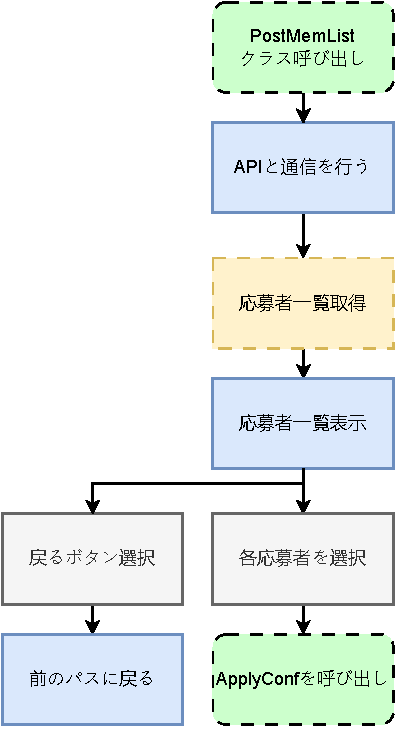
\includegraphics[width=7cm]{./images/internal-design/state_change_diagram/mypage/post_member_list.pdf}
  \caption{post\_mem\_list.dartの状態遷移図}
\end{figure}


\clearpage

\begin{table}[H]
  \centering
  \begin{tabular}{|c|l|l|} \hline
    モジュール名                & \multicolumn{2}{l|}{impressions.dart}                                                                                  \\ \hline
    モジュール概要               & \multicolumn{2}{p{12cm}|}{法人利用者が投稿を行った広告のインプレッション情報を閲覧できる画面を表示するモジュール}                                                 \\ \hline
    責任者                   & \multicolumn{2}{l|}{新谷光城}                                                                                              \\ \hline
    \multirow{7}{*}{構成要素} & クラス名                                                                   & Impressios                                    \\ \cline{2-3}
                          & クラス種類                                                                  & extends StatelessWidget                       \\ \cline{2-3}
                          & 処理概要                                                                   & \multicolumn{1}{p{12cm}|}{インプレッション画面を表示するクラス} \\ \cline{2-3}
                          & 入力                                                                     & Map$<$String, dynamic $>$ impressions         \\ \cline{2-3}
                          & 出力                                                                     & Widget                                        \\ \cline{2-3}
                          & \multicolumn{2}{l|}{他クラス・関数との関係}                                                                                       \\ \cline{2-3}
                          & \multicolumn{2}{p{14cm}|}{戻るボタンの選択で前のモジュールに戻る}                                                                         \\ \hline
  \end{tabular}
\end{table}

\begin{figure}[H]
  \centering
  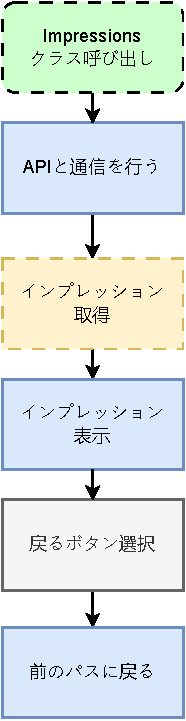
\includegraphics[width=4cm]{./images/internal-design/state_change_diagram/mypage/impressions.pdf}
  \caption{impressions.dartの状態遷移図}
\end{figure}


\begin{table}[H]
  \centering
  \begin{tabular}{|c|l|l|} \hline
    モジュール名 & \multicolumn{2}{l|}{login\_page.dart} \\ \hline
    モジュール概要 & \multicolumn{2}{p{12cm}|}{ログイン画面を生成するモジュール} \\ \hline
    責任者 & \multicolumn{2}{l|}{山本昇永} \\ \hline
    \multirow{7}{*}{構成要素} & クラス名 & LoginPage \\ \cline{2-3}
                            & クラス種類 & extends StatelessWidget \\ \cline{2-3}
                            & 処理概要 & \multicolumn{1}{p{12cm}|}{ログイン画面のWidgetを動的に変更するクラス} \\ \cline{2-3}
                            & 入力 & なし \\ \cline{2-3}
                            & 出力 & Widget \\ \cline{2-3}
                            & \multicolumn{2}{l|}{他クラス・関数との関係} \\ \cline{2-3}
                            & \multicolumn{2}{p{14cm}|}{login\_page.dartのLoginPageStateクラスを組み込む} \\ \hline
    \multirow{7}{*}{構成要素} & クラス名 & LoginPageState \\ \cline{2-3}
                            & クラス種類 & extends StatelessWidget \\ \cline{2-3}
                            & 処理概要 & \multicolumn{1}{p{12cm}|}{ログイン画面の状態を返すクラス} \\ \cline{2-3}
                            & 入力 & なし \\ \cline{2-3}
                            & 出力 & State \\ \cline{2-3}
                            & \multicolumn{2}{l|}{他クラス・関数との関係} \\ \cline{2-3}
                            & \multicolumn{2}{p{14cm}|}{
                            new\_menber\_company.dartのNewMemberGeneralクラスを呼び出すことで、一般用の新規会員登録画面を表示
                            \newline new\_member\_general.dartのNewMemberGeneralクラスを呼び出すことで、法人用の新規会員登録画面を表示
                            \newline pass\_change.dartのPassChangeクラスを呼び出すことで、パスワード再登録画面を表示
                            \newline ask\_page.dartのAskPageクラスを呼び出すことで、お問い合わせ画面を表示
                            \newline login\_page.dartのLoginAppBarクラスを組み込む
                            \newline change\_generalcorporation.dartのChangeGeneralCorporationプロバイダを組み込む} \\ \hline
    \multirow{7}{*}{構成要素} & クラス名 & LoginAppBar \\ \cline{2-3}
                            & クラス種類 & extends StatelessWidget, imprements PrefferdSizeWidget \\ \cline{2-3}
                            & 処理概要 & \multicolumn{1}{p{12cm}|}{ログイン画面用に作成を行ったAppBarを生成するコンポーネント} \\ \cline{2-3}
                            & 入力 & ChangeGeneralCorporation store \\ \cline{2-3}
                            & 出力 & Widget \\ \cline{2-3}
                            & \multicolumn{2}{l|}{他クラス・関数との関係} \\ \cline{2-3}
                            & \multicolumn{2}{p{14cm}|}{なし} \\ \hline
  \end{tabular}
\end{table}

\begin{table}[H]
  \centering
  \begin{tabular}{|c|l|l|} \hline
    モジュール名 & \multicolumn{2}{l|}{new\_member\_company.dart} \\ \hline
    モジュール概要 & \multicolumn{2}{p{12cm}|}{法人用の新規会員登録画面を生成するモジュール} \\ \hline
    責任者 & \multicolumn{2}{l|}{山本昇永} \\ \hline
    \multirow{7}{*}{構成要素} & クラス名 & NewMemberCompany \\ \cline{2-3}
                            & クラス種類 & extends StatelessWidget \\ \cline{2-3}
                            & 処理概要 & \multicolumn{1}{p{12cm}|}{法人用の新規会員登録画面のWidgetを動的に変更するクラス} \\ \cline{2-3}
                            & 入力 & なし \\ \cline{2-3}
                            & 出力 & Widget \\ \cline{2-3}
                            & \multicolumn{2}{l|}{他クラス・関数との関係} \\ \cline{2-3}
                            & \multicolumn{2}{p{14cm}|}{new\_menber\_company.dartのNewMenberCompanyStateクラスを組み込む} \\ \hline
    \multirow{7}{*}{構成要素} & クラス名 & NewMemberCompanyState \\ \cline{2-3}
                            & クラス種類 & extends StatelessWidget \\ \cline{2-3}
                            & 処理概要 & \multicolumn{1}{p{12cm}|}{法人用の新規会員登録画面の状態を返すクラス} \\ \cline{2-3}
                            & 入力 & なし \\ \cline{2-3}
                            & 出力 & State \\ \cline{2-3}
                            & \multicolumn{2}{l|}{他クラス・関数との関係} \\ \cline{2-3}
                            & \multicolumn{2}{p{14cm}|}{
                            rule\_scree.dartのRuleScreenクラスを呼び出すことで利用規約を表示
                            \newline finish\_screen.dartのFinishScreenクラス呼び出すことで新規会員登録完了画面を表示
                            \newline title\_appbar.dartのTitleAppBarクラスを組み込む
                            \newline password\_input.dartのPasswordInputクラスを組み込む
                            \newline normal\_bottom\_apbar.dartクラスを組み込む
                            \newline new\_menber\_company.dartのTextEnterBoxクラスを組み込む
                            \newline change\_generalcorporation.dartのChangeGeneralCorporationプロバイダを組み込む
                            \newline 戻るボタンの選択で前のモジュールに戻る} \\ \hline
    \multirow{7}{*}{構成要素} & クラス名 & TextEnterBox \\ \cline{2-3}
                            & クラス種類 & extends StatelessWidget \\ \cline{2-3}
                            & 処理概要 & \multicolumn{1}{p{12cm}|}{入力フォームを生成するコンポーネント} \\ \cline{2-3}
                            & 入力 & String label, String guide, double width \\ \cline{2-3}
                            & 出力 & Widget \\ \cline{2-3}
                            & \multicolumn{2}{l|}{他クラス・関数との関係} \\ \cline{2-3}
                            & \multicolumn{2}{p{14cm}|}{なし} \\ \hline
    \multirow{7}{*}{構成要素} & クラス名 & PasswordInput \\ \cline{2-3}
                            & クラス種類 & extends StatelessWidget \\ \cline{2-3}
                            & 処理概要 & \multicolumn{1}{p{12cm}|}{パスワード入力フォームのWidgetを動的に変更するクラス} \\ \cline{2-3}
                            & 入力 & String label, bool is\_show, ValueChange$<$bool$>$ \\ \cline{2-3}
                            & 出力 & Widget \\ \cline{2-3}
                            & \multicolumn{2}{l|}{他クラス・関数との関係} \\ \cline{2-3}
                            & \multicolumn{2}{p{14cm}|}{} \\ \hline
    \multirow{7}{*}{構成要素} & クラス名 & PasswordInputState \\ \cline{2-3}
                            & クラス種類 & extends StatelessWidget \\ \cline{2-3}
                            & 処理概要 & \multicolumn{1}{p{12cm}|}{パスワード入力フォームの状態を返すクラス} \\ \cline{2-3}
                            & 入力 & なし \\ \cline{2-3}
                            & 出力 & State \\ \cline{2-3}
                            & \multicolumn{2}{l|}{他クラス・関数との関係} \\ \cline{2-3}
                            & \multicolumn{2}{p{14cm}|}{なし} \\ \hline
  \end{tabular}
\end{table}

\begin{table}[H]
  \centering
  \begin{tabular}{|c|l|l|} \hline
    モジュール名 & \multicolumn{2}{l|}{new\_menber\_general.dart} \\ \hline
    モジュール概要 & \multicolumn{2}{p{12cm}|}{一般用の新規会員登録画面を生成するモジュール} \\ \hline
    責任者 & \multicolumn{2}{l|}{山本昇永} \\ \hline
    \multirow{7}{*}{構成要素} & クラス名 & NewMenberGeneral \\ \cline{2-3}
                            & クラス種類 & extends StatelessWidget \\ \cline{2-3}
                            & 処理概要 & \multicolumn{1}{p{12cm}|}{一般用の新規会員登録画面のWidgetを動的に変更するクラス} \\ \cline{2-3}
                            & 入力 & なし \\ \cline{2-3}
                            & 出力 & Widget \\ \cline{2-3}
                            & \multicolumn{2}{l|}{他クラス・関数との関係} \\ \cline{2-3}
                            & \multicolumn{2}{p{14cm}|}{new\_menber\_general.dartのNewMenberGeneralStateクラスを組み込む} \\ \hline
    \multirow{7}{*}{構成要素} & クラス名 & NewMenberGeneralState \\ \cline{2-3}
                            & クラス種類 & extends StatelessWidget \\ \cline{2-3}
                            & 処理概要 & \multicolumn{1}{p{12cm}|}{一般用の新規会員登録画面の状態を返すクラス} \\ \cline{2-3}
                            & 入力 & なし \\ \cline{2-3}
                            & 出力 & State \\ \cline{2-3}
                            & \multicolumn{2}{l|}{他クラス・関数との関係} \\ \cline{2-3}
                            & \multicolumn{2}{p{14cm}|}{
                            rule\_scree.dartのRuleScreenクラスを呼び出すことで利用規約を表示
                            \newline finish\_screen.dartのFinishScreenクラス呼び出すことで新規会員登録完了画面を表示
                            \newline title\_appbar.dartのTitleAppBarクラスを組み込む
                            \newline password\_input.dartのPasswordInputクラスを組み込む
                            \newline normal\_bottom\_apbar.dartクラスを組み込む
                            \newline change\_generalcorporation.dartのChangeGeneralCorporationプロバイダを組み込む
                            \newline 戻るボタンの選択で前のモジュールに戻る} \\ \hline
  \end{tabular}
\end{table}

\begin{table}[H]
  \centering
  \begin{tabular}{|c|l|l|} \hline
    モジュール名 & \multicolumn{2}{l|}{pass\_change.dart} \\ \hline
    モジュール概要 & \multicolumn{2}{p{12cm}|}{パスワード再設定画面を生成するモジュール} \\ \hline
    責任者 & \multicolumn{2}{l|}{金川幸太} \\ \hline
    \multirow{7}{*}{構成要素} & クラス名 & PassChange \\ \cline{2-3}
                            & クラス種類 & extends StatelessWidget \\ \cline{2-3}
                            & 処理概要 & \multicolumn{1}{p{12cm}|}{パスワード再設定画面のWidgetを動的に変更するクラス} \\ \cline{2-3}
                            & 入力 & なし \\ \cline{2-3}
                            & 出力 & Widget \\ \cline{2-3}
                            & \multicolumn{2}{l|}{他クラス・関数との関係} \\ \cline{2-3}
                            & \multicolumn{2}{p{14cm}|}{pass\_change.dartのPassChangeStateクラスを組み込む} \\ \hline
    \multirow{7}{*}{構成要素} & クラス名 & PassChangeState \\ \cline{2-3}
                            & クラス種類 & extends StatelessWidget \\ \cline{2-3}
                            & 処理概要 & \multicolumn{1}{p{12cm}|}{パスワード再設定画面の状態を返すクラス} \\ \cline{2-3}
                            & 入力 & なし \\ \cline{2-3}
                            & 出力 & State \\ \cline{2-3}
                            & \multicolumn{2}{l|}{他クラス・関数との関係} \\ \cline{2-3}
                            & \multicolumn{2}{p{14cm}|}{
                            finish\_screen.dartのFinishScreenクラスを呼び出すことでパスワード再設定完了画面を表示
                            \newline change\_generalcorporation.dartのChangeGeneralCorporationプロバイダを組み込む
                            \newline title\_appbar.dartのTitleAppBarクラスを組み込む
                            \newline normal\_bottom\_apbar.dartクラスを組み込む
                            \newline 戻るボタンの選択で前のモジュールに戻る} \\ \hline
  \end{tabular}
\end{table}

\begin{table}[H]
  \centering
  \begin{tabular}{|c|l|l|} \hline
    モジュール名 & \multicolumn{2}{l|}{ask\_page.dart} \\ \hline
    モジュール概要 & \multicolumn{2}{p{12cm}|}{問い合わせ画面を生成するモジュール} \\ \hline
    責任者 & \multicolumn{2}{l|}{金川幸太} \\ \hline
    \multirow{7}{*}{構成要素} & クラス名 & AskPage \\ \cline{2-3}
                            & クラス種類 & extends StatelessWidget \\ \cline{2-3}
                            & 処理概要 & \multicolumn{1}{p{12cm}|}{問い合わせ画面のWidgetを動的に変更するクラス} \\ \cline{2-3}
                            & 入力 & bool is\_login \\ \cline{2-3}
                            & 出力 & Widget \\ \cline{2-3}
                            & \multicolumn{2}{l|}{他クラス・関数との関係} \\ \cline{2-3}
                            & \multicolumn{2}{p{14cm}|}{ask\_page.dartのAskPageStateクラスを組み込む} \\ \hline
    \multirow{7}{*}{構成要素} & クラス名 & AskPageState \\ \cline{2-3}
                            & クラス種類 & extends StatelessWidget \\ \cline{2-3}
                            & 処理概要 & \multicolumn{1}{p{12cm}|}{問い合わせ画面の状態を返すクラス} \\ \cline{2-3}
                            & 入力 & なし \\ \cline{2-3}
                            & 出力 & State \\ \cline{2-3}
                            & \multicolumn{2}{l|}{他クラス・関数との関係} \\ \cline{2-3}
                            & \multicolumn{2}{p{14cm}|}{
                            comment\_box.dartのCommentBoxクラスの組み込み
                            \newline finish\_screen.dartのFinishScreenクラスを呼び出すことで問い合わせ完了画面を表示
                            \newline change\_generalcorporation.dartのChangeGeneralCorporationプロバイダを組み込む
                            \newline title\_appbar.dartのTitleAppBarクラスを組み込む
                            \newline normal\_bottom\_apbar.dartクラスを組み込む
                            \newline 戻るボタンの選択で前のモジュールに戻る} \\ \hline
  \end{tabular}
\end{table}
\clearpage
\subsubsection{job}
\begin{table}[H]
  \centering
  \begin{tabular}{|c|l|l|} \hline
    モジュール名                & \multicolumn{2}{l|}{job.dart}                                                                         \\ \hline
    モジュール概要               & \multicolumn{2}{p{12cm}|}{求人画面を表示するモジュール}                                                             \\ \hline
    責任者                   & \multicolumn{2}{l|}{新谷光城}                                                                             \\ \hline
    \multirow{7}{*}{構成要素} & クラス名                                                 & JobRouterPage                                  \\ \cline{2-3}
                          & クラス種類                                                & extends AppRouter                              \\ \cline{2-3}
                          & 処理概要                                                 & \multicolumn{1}{p{12cm}|}{JobをアクセスするためのRouter} \\ \cline{2-3}
                          & 入力                                                   & なし                                             \\ \cline{2-3}
                          & 出力                                                   & Route                                          \\ \cline{2-3}
                          & \multicolumn{2}{l|}{他クラス・関数との関係}                                                                      \\ \cline{2-3}
                          & \multicolumn{2}{p{14cm}|}{なし}                                                                         \\ \hline
    \multirow{7}{*}{構成要素} & クラス名                                                 & Job                                            \\ \cline{2-3}
                          & クラス種類                                                & extends StatelessWidget                        \\ \cline{2-3}
                          & 処理概要                                                 & \multicolumn{1}{p{12cm}|}{求人画面を動的にするクラス}       \\ \cline{2-3}
                          & 入力                                                   & なし                                             \\ \cline{2-3}
                          & 出力                                                   & Widget                                         \\ \cline{2-3}
                          & \multicolumn{2}{l|}{他クラス・関数との関係}                                                                      \\ \cline{2-3}
                          & \multicolumn{2}{p{14cm}|}{job.dartのJobStateクラスを組み込む}                                                  \\ \hline
    \multirow{7}{*}{構成要素} & クラス名                                                 & JobState                                       \\ \cline{2-3}
                          & クラス種類                                                & extends StatelessWidget                        \\ \cline{2-3}
                          & 処理概要                                                 & \multicolumn{1}{p{12cm}|}{求人画面の状態を返すクラス}       \\ \cline{2-3}
                          & 入力                                                   & なし                                             \\ \cline{2-3}
                          & 出力                                                   & State                                          \\ \cline{2-3}
                          & \multicolumn{2}{l|}{他クラス・関数との関係}                                                                      \\ \cline{2-3}
                          & \multicolumn{2}{p{14cm}|}{
      post\_list.dartのPostListクラスを組み込む
      \newline else\_list.dartのElseListクラスを呼び出すことでお気に入りイベント一覧画面、閲覧履歴画面を表示
      \newline search\_post.dartのSearchPostを呼び出すことで検索結果画面を表示
    \newline job\_post\_write.dartのJobPostWriteクラスを呼び出すことで求人詳細画面を表示}                                                              \\ \hline
  \end{tabular}
\end{table}

\begin{figure}[H]
  \centering
  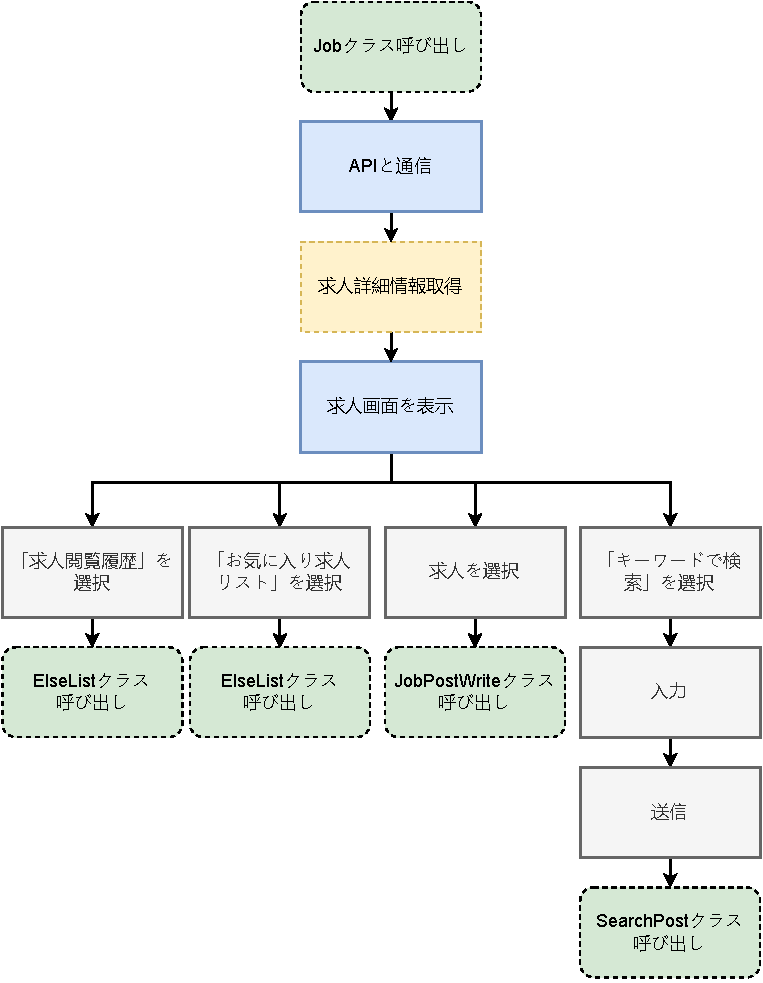
\includegraphics[width=16cm]{./images/internal-design/state_change_diagram/job/job.pdf}
  \caption{job.dartの状態遷移図}
\end{figure}


\begin{table}[H]
  \centering
  \begin{tabular}{|c|l|l|} \hline
    モジュール名                & \multicolumn{2}{l|}{job\_post\_write.dart}                                                        \\ \hline
    モジュール概要               & \multicolumn{2}{p{12cm}|}{イベント広告内容記述画面を表示するモジュール}                                                 \\ \hline
    責任者                   & \multicolumn{2}{l|}{新谷光城}                                                                         \\ \hline
    \multirow{7}{*}{構成要素} & クラス名                                              & JobPostWrite                                  \\ \cline{2-3}
                          & クラス種類                                             & extends StatelessWidget                       \\ \cline{2-3}
                          & 処理概要                                              & \multicolumn{1}{p{12cm}|}{求人広告内容記述画面を表示するクラス} \\ \cline{2-3}
                          & 入力                                                & なし                                            \\ \cline{2-3}
                          & 出力                                                & Widget                                        \\ \cline{2-3}
                          & \multicolumn{2}{l|}{他クラス・関数との関係}                                                                  \\ \cline{2-3}
                          & \multicolumn{2}{p{14cm}|}{
      change\_general\_corporation.dartのChangeGeneralCorporationプロバイダを組み込む
      \newline job\_fee\_select.dartのJobPostInfoプロバイダを組み込む
      \newline title\_appbar.dartのTitleAppBarクラスを組み込む
      \newline post\_conf.dartのPostConfクラスを呼び出し投稿確認オーバーレイを表示
      \newline return\_write.dartのReturnWriteクラスを呼び出し必須内容記入漏れ注意オーバーレイを表示
      \newline move\_conf.dartのMoveConfクラスを呼び出し投稿中に移動確認オーバーレイを表示
    \newline 戻るボタンの選択で前のモジュールに戻る}                                                                                             \\ \hline
  \end{tabular}
\end{table}

\begin{figure}[H]
  \centering
  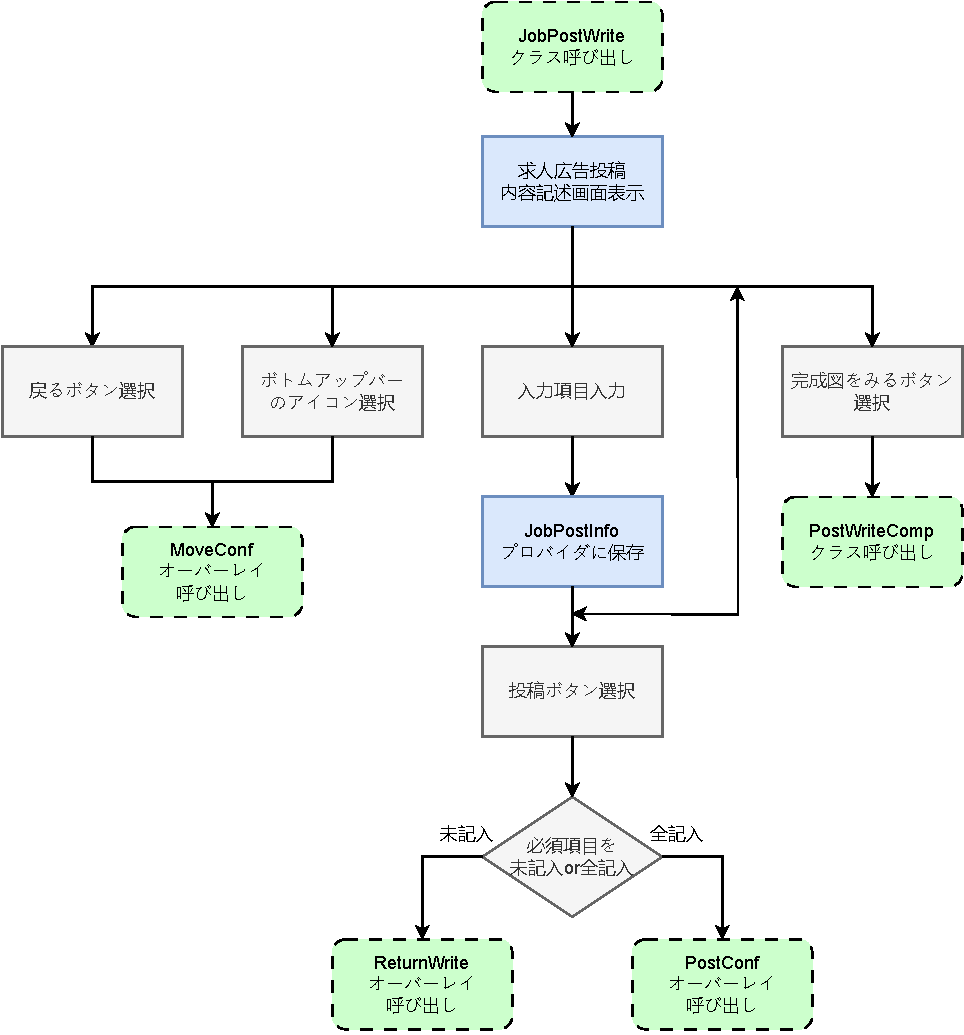
\includegraphics[width=17cm]{./images/internal-design/state_change_diagram/job/job_post_write.pdf}
  \caption{job\_post\_write.dartの状態遷移図}
\end{figure}




\begin{table}[H]
  \centering
  \begin{tabular}{|c|l|l|} \hline
    モジュール名                & \multicolumn{2}{l|}{job\_post\_detail.dart}                                                                              \\ \hline
    モジュール概要               & \multicolumn{2}{p{12cm}|}{求人広告詳細画面を表示するモジュール}                                                                            \\ \hline
    責任者                   & \multicolumn{2}{l|}{新谷光城}                                                                                                \\ \hline
    \multirow{7}{*}{構成要素} & クラス名                                                                    & JobPostDetail                                  \\ \cline{2-3}
                          & クラス種類                                                                   & extends StatelessWidget                        \\ \cline{2-3}
                          & 処理概要                                                                    & \multicolumn{1}{p{12cm}|}{求人広告詳細画面を動的に変更するクラス} \\ \cline{2-3}
                          & 入力                                                                      & Map$<$String, dynamic$>$ info                  \\ \cline{2-3}
                          & 出力                                                                      & Widget                                         \\ \cline{2-3}
                          & \multicolumn{2}{l|}{他クラス・関数との関係}                                                                                         \\ \cline{2-3}
                          & \multicolumn{2}{p{14cm}|}{job\_post\_detail.dartのJobPostDetailクラスを組み込む}                                                  \\ \hline
    \multirow{7}{*}{構成要素} & クラス名                                                                    & JobPostDetailState                             \\ \cline{2-3}
                          & クラス種類                                                                   & extends StatelessWidget                        \\ \cline{2-3}
                          & 処理概要                                                                    & \multicolumn{1}{p{12cm}|}{求人広告詳細画面の状態を返すクラス}   \\ \cline{2-3}
                          & 入力                                                                      & なし                                             \\ \cline{2-3}
                          & 出力                                                                      & State                                          \\ \cline{2-3}
                          & \multicolumn{2}{l|}{他クラス・関数との関係}                                                                                         \\ \cline{2-3}
                          & \multicolumn{2}{p{14cm}|}{
      change\_general\_corporation.dartのChangeGeneralCorporationプロバイダを組み込む
      \newline title\_appbar.dartのTitleAppBarクラスを組み込む
      \newline impression.dartのImpressionクラスを呼び出しインプレッション画面を表示
      \newline post\_mem\_list.dartのPostMemListクラスを呼び出し応募者一覧画面を表示
      \newline event\_post\_write.dartのEventPostWriteクラスを呼び出しイベント広告内容変更画面を表示
    \newline delete\_conf.dartのDeleteConfクラスを呼び出し投稿削除確認オーバーレイを表示}                                                                                    \\ \hline
  \end{tabular}
\end{table}

\begin{figure}[H]
  \centering
  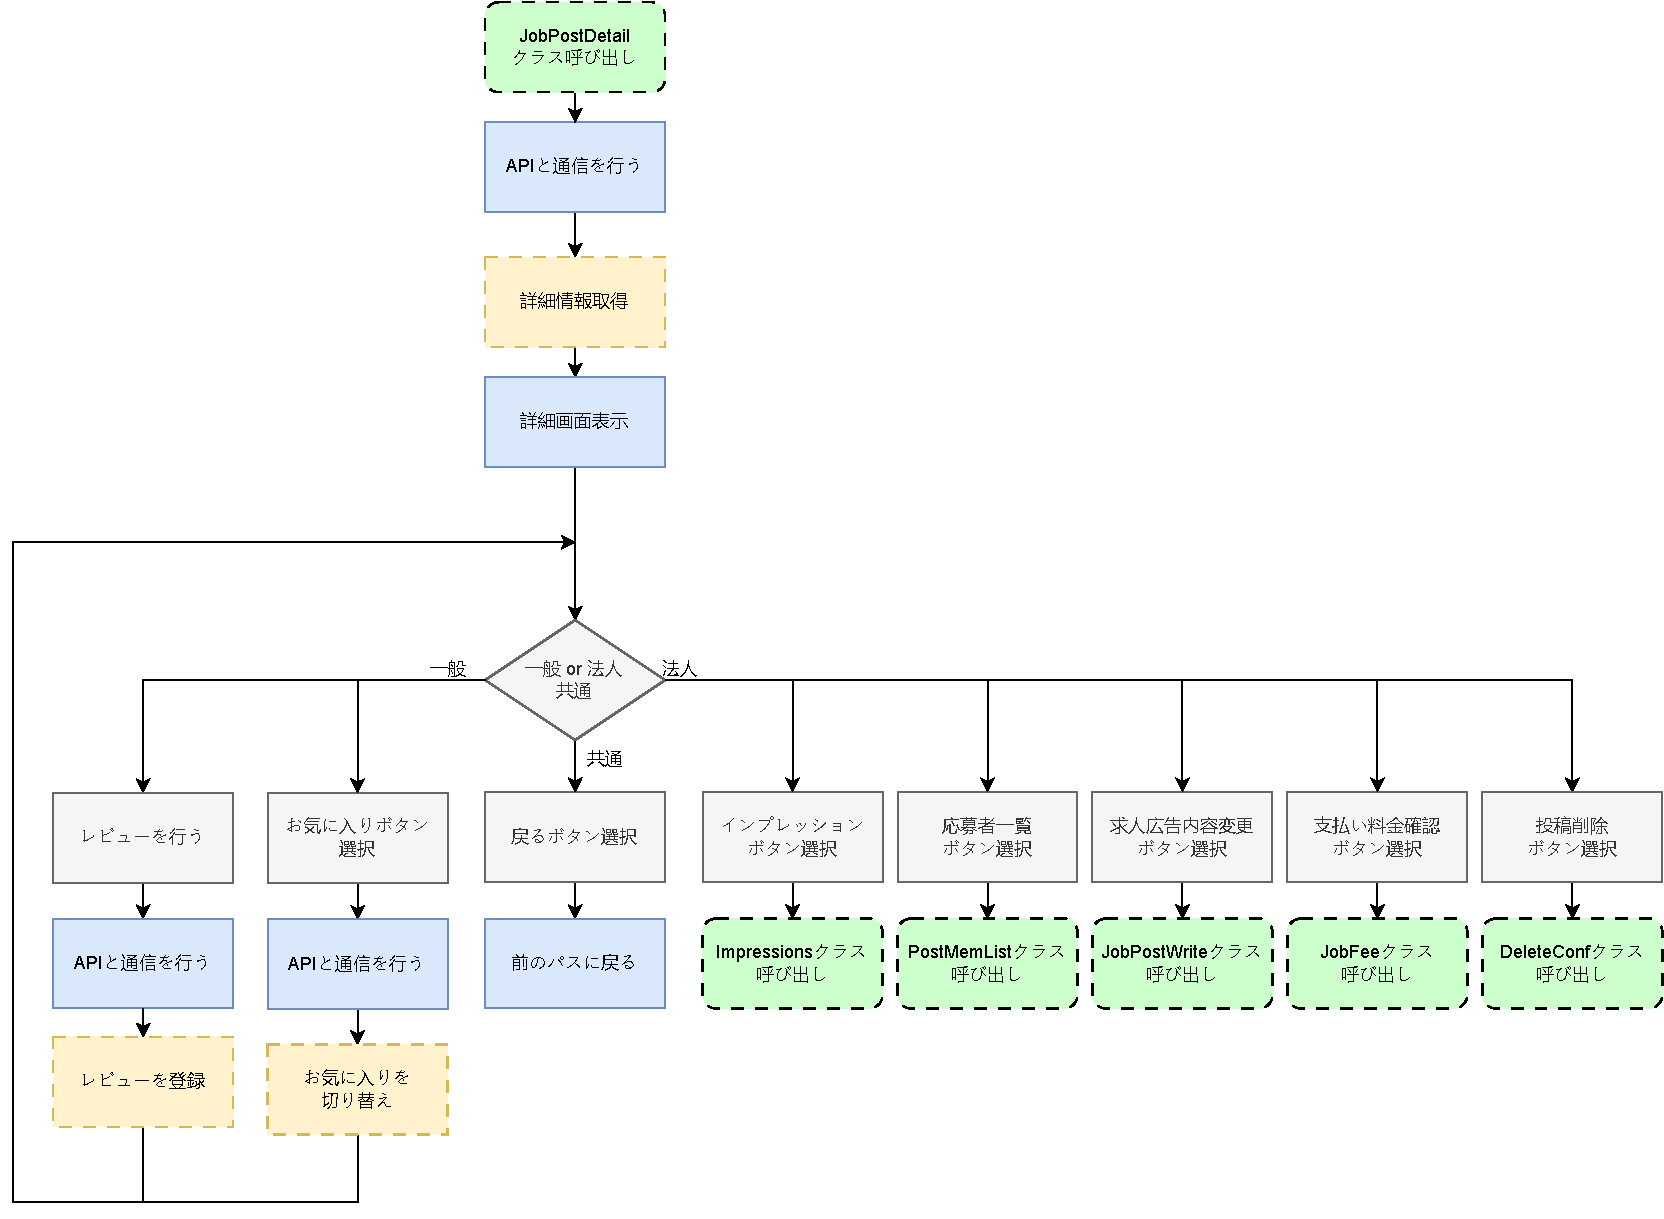
\includegraphics[width=18cm]{./images/internal-design/state_change_diagram/job/job_post_detail.pdf}
  \caption{job\_post\_detail.dartの状態遷移図}
\end{figure}
\begin{table}[H]
  \centering
  \begin{tabular}{|c|l|l|} \hline
    モジュール名                & \multicolumn{2}{l|}{home.dart}                                                                                                                   \\ \hline
    モジュール概要               & \multicolumn{2}{p{12cm}|}{ホーム画面を作成するモジュール}                                                                                                       \\ \hline
    責任者                   & \multicolumn{2}{l|}{新谷光城}                                                                                                                        \\ \hline
    \multirow{7}{*}{構成要素} & クラス名                                                                                & HomeRouterPage                                             \\ \cline{2-3}
                          & クラス種類                                                                               & extends AppRouter                                          \\ \cline{2-3}
                          & 処理概要                                                                                & \multicolumn{1}{p{12cm}|}{HomeをアクセスするためのRouter}            \\ \cline{2-3}
                          & 入力                                                                                  & なし                                                         \\ \cline{2-3}
                          & 出力                                                                                  & Route                                                      \\ \cline{2-3}
                          & \multicolumn{2}{l|}{他クラス・関数との関係}                                                                                                                 \\ \cline{2-3}
                          & \multicolumn{2}{p{14cm}|}{なし}                                                                                                                    \\ \hline
    \multirow{7}{*}{構成要素} & クラス名                                                                                & Home                                                       \\ \cline{2-3}
                          & クラス種類                                                                               & extends StatelessWidget                                    \\ \cline{2-3}
                          & 処理概要                                                                                & \multicolumn{1}{p{12cm}|}{ホーム画面のWidgetを動的に変更するクラス}         \\ \cline{2-3}
                          & 入力                                                                                  & なし                                                         \\ \cline{2-3}
                          & 出力                                                                                  & Widget                                                     \\ \cline{2-3}
                          & \multicolumn{2}{l|}{他クラス・関数との関係}                                                                                                                 \\ \cline{2-3}
                          & \multicolumn{2}{p{14cm}|}{home.dartのHomeStateクラスを組み込む}                                                                                           \\ \hline
    \multirow{7}{*}{構成要素} & クラス名                                                                                & HomeState                                                  \\ \cline{2-3}
                          & クラス種類                                                                               & extends StatelessWidget                                    \\ \cline{2-3}
                          & 処理概要                                                                                & \multicolumn{1}{p{12cm}|}{ホーム画面の状態を返すクラス}                  \\ \cline{2-3}
                          & 入力                                                                                  & なし                                                         \\ \cline{2-3}
                          & 出力                                                                                  & State                                                      \\ \cline{2-3}
                          & \multicolumn{2}{l|}{他クラス・関数との関係}                                                                                                                 \\ \cline{2-3}
                          & \multicolumn{2}{p{14cm}|}{
      home.dartのMainAppBarクラスを組み込む
      \newline change\_general\_corporation.dartのChangeGeneralCorporationプロバイダを組み込む
      \newline else\_list.dartのElseListクラスを呼び出すことで閲覧履歴画面を表示
    \newline post\_list.dartのPostListクラスを呼び出すことで閲覧履歴詳細画面を表示}                                                                                                                 \\ \hline
    \multirow{7}{*}{構成要素} & クラス名                                                                                & MainAppBar                                                 \\ \cline{2-3}
                          & クラス種類                                                                               & extends StatelessWidget, imprements PreferredSizeWidget    \\ \cline{2-3}
                          & 処理概要                                                                                & \multicolumn{1}{p{12cm}|}{ホーム画面用に作成を行ったAppBarを生成するコンポーネント} \\ \cline{2-3}
                          & 入力                                                                                  & Widget component                                           \\ \cline{2-3}
                          & 出力                                                                                  & Widget                                                     \\ \cline{2-3}
                          & \multicolumn{2}{l|}{他クラス・関数との関係}                                                                                                                 \\ \cline{2-3}
                          & \multicolumn{2}{p{14cm}|}{notice.dartのNoticeクラスを呼び出し通知画面を表示}                                                                                     \\ \hline
    \multirow{7}{*}{構成要素} & クラス名                                                                                & GeneralHomeButton                                          \\ \cline{2-3}
                          & クラス種類                                                                               & extends StatelessWidget                                    \\ \cline{2-3}
                          & 処理概要                                                                                & \multicolumn{1}{p{12cm}|}{一般利用者用画面でのボタンを生成するコンポーネント}       \\ \cline{2-3}
                          & 入力                                                                                  & なし                                                         \\ \cline{2-3}
                          & 出力                                                                                  & Widget                                                     \\ \cline{2-3}
                          & \multicolumn{2}{l|}{他クラス・関数との関係}                                                                                                                 \\ \cline{2-3}
                          & \multicolumn{2}{p{14cm}|}{else\_list.dartのElseListクラスを呼び出すことで応募履歴一覧画面、お気に入り一覧画面を表示}                                                              \\
    \hline
    \multirow{7}{*}{構成要素} & クラス名                                                                                & CompanyHomeButton                                          \\ \cline{2-3}
                          & クラス種類                                                                               & extends StatelessWidget                                    \\ \cline{2-3}
                          & 処理概要                                                                                & \multicolumn{1}{p{12cm}|}{法人利用者用画面でのボタンを生成するコンポーネント}       \\ \cline{2-3}
                          & 入力                                                                                  & なし                                                         \\ \cline{2-3}
                          & 出力                                                                                  & Widget                                                     \\ \cline{2-3}
                          & \multicolumn{2}{l|}{他クラス・関数との関係}                                                                                                                 \\ \cline{2-3}
                          & \multicolumn{2}{p{14cm}|}{
      else\_list.dartのElseListクラスを呼び出すことで応募履歴一覧画面、お気に入り一覧画面を表示
    \newline posted\_list.dartのPostedListクラスを呼び出すことで投稿広告一覧画面を表示}                                                                                                             \\ \hline
  \end{tabular}
\end{table}

\begin{figure}[H]
  \centering
  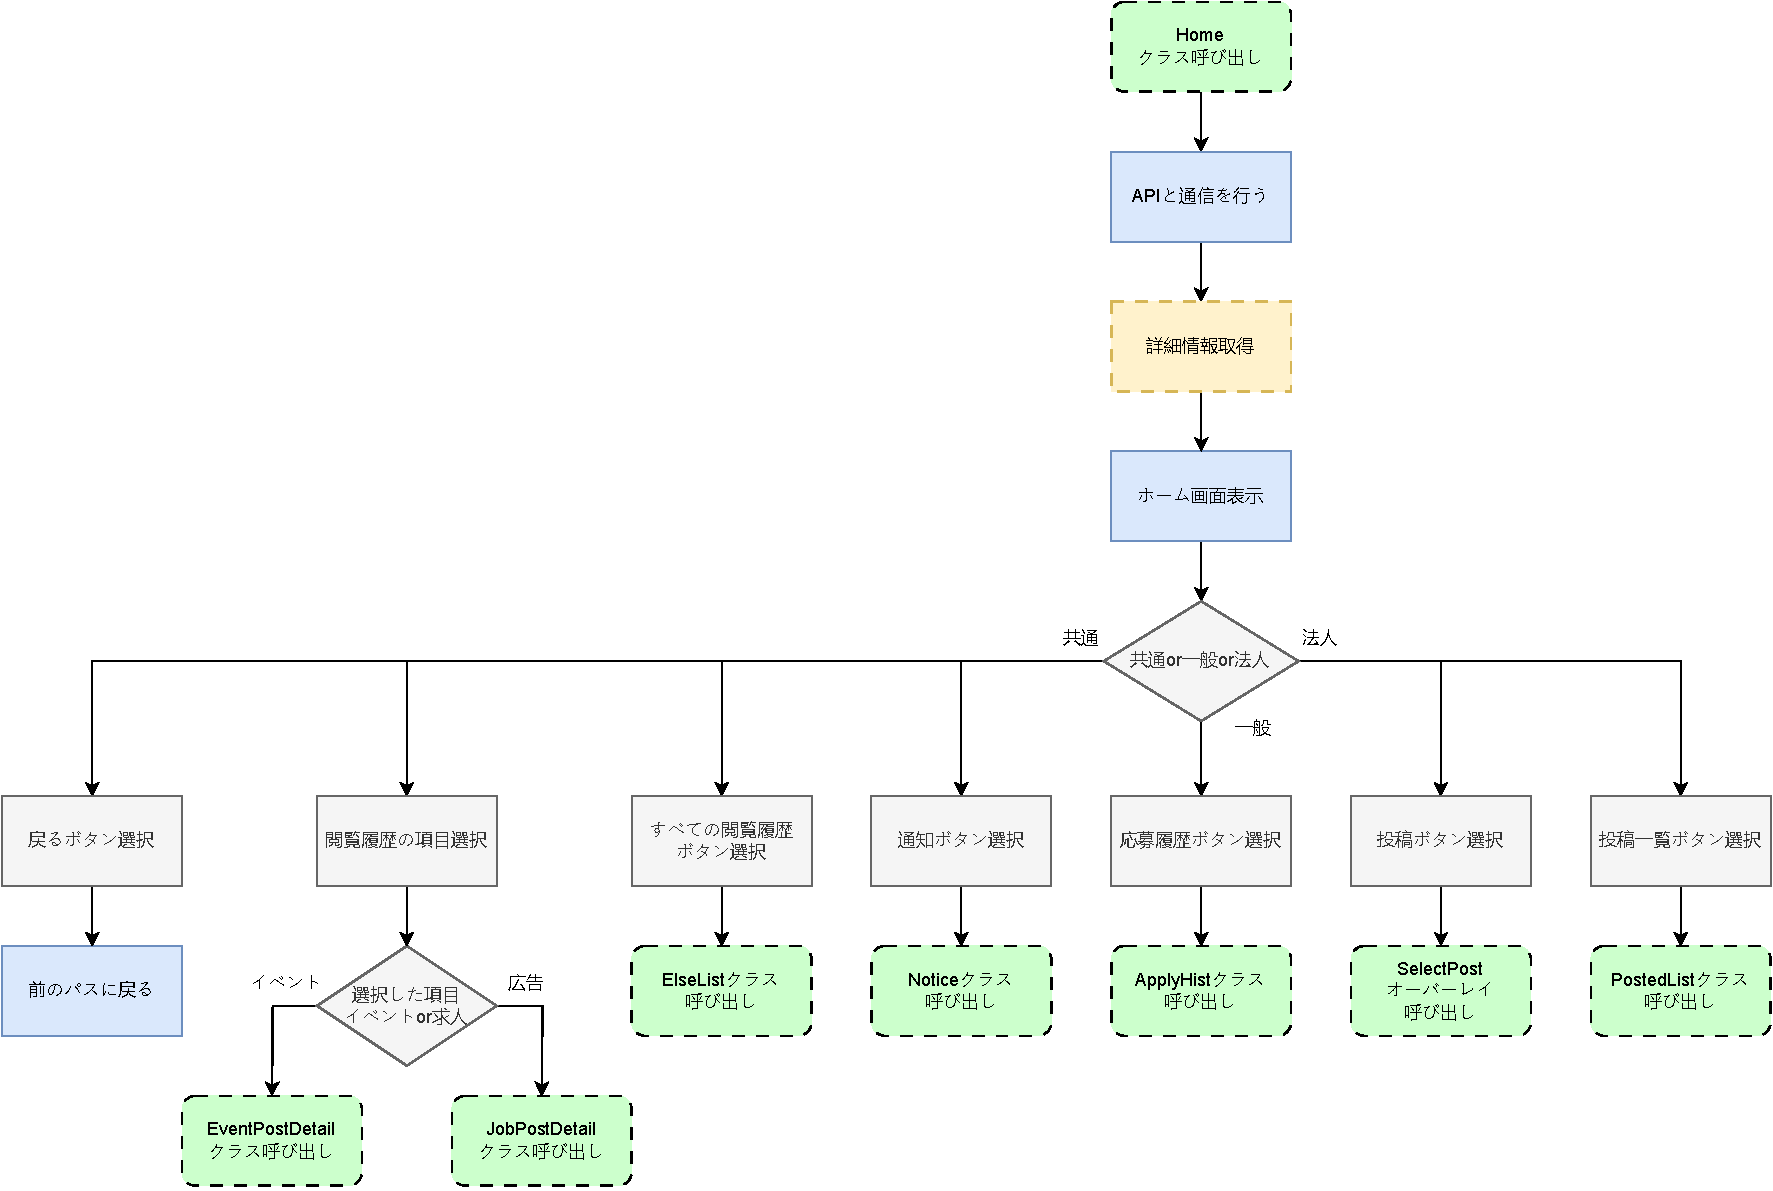
\includegraphics[width=15cm]{./images/internal-design/state_change_diagram/home/home.pdf}
  \caption{home.dartの状態遷移図}
\end{figure}

\begin{table}[H]
  \centering
  \begin{tabular}{|c|l|l|} \hline
    モジュール名                & \multicolumn{2}{l|}{notice.dart}                                                                                                               \\ \hline
    モジュール概要               & \multicolumn{2}{p{12cm}|}{通知画面を作成するモジュール}                                                                                                      \\ \hline
    責任者                   & \multicolumn{2}{l|}{新谷光城}                                                                                                                      \\ \hline
    \multirow{7}{*}{構成要素} & クラス名                                                       & Notice                                                                            \\ \cline{2-3}
                          & クラス種類                                                      & extends StatelessWidget                                                           \\ \cline{2-3}
                          & 処理概要                                                       & \multicolumn{1}{p{12cm}|}{通知画面のWidgetを動的に変更するクラス}                                 \\ \cline{2-3}
                          & 入力                                                         & なし                                                                                \\ \cline{2-3}
                          & 出力                                                         & Widget                                                                            \\ \cline{2-3}
                          & \multicolumn{2}{l|}{他クラス・関数との関係}                                                                                                               \\ \cline{2-3}
                          & \multicolumn{2}{p{14cm}|}{notice.dartのNoticeStateクラスを組み込む}                                                                                     \\ \hline
    \multirow{7}{*}{構成要素} & クラス名                                                       & NoticeState                                                                       \\ \cline{2-3}
                          & クラス種類                                                      & extends StatelessWidget                                                           \\ \cline{2-3}
                          & 処理概要                                                       & \multicolumn{1}{p{12cm}|}{通知画面の状態を返すクラス}                                          \\ \cline{2-3}
                          & 入力                                                         & なし                                                                                \\ \cline{2-3}
                          & 出力                                                         & State                                                                             \\ \cline{2-3}
                          & \multicolumn{2}{l|}{他クラス・関数との関係}                                                                                                               \\ \cline{2-3}
                          & \multicolumn{2}{p{14cm}|}{
      notice.dartのNoticeListViewクラスを組み込む
      \newline change\_general\_corporation.dartのChangeGeneralCorporationプロバイダを組み込む
      \newline title\_appbar.dartのTitleAppBarクラスを組み込む
    \newline toggle\_button.dartのToggleButtonクラスを組み込む}                                                                                                                     \\ \hline
    \multirow{7}{*}{構成要素} & クラス名                                                       & NoticeListView                                                                    \\ \cline{2-3}
                          & クラス種類                                                      & extends StatelessWidget                                                           \\ \cline{2-3}
                          & 処理概要                                                       & \multicolumn{1}{p{12cm}|}{通知の一覧を生成するクラス}                                          \\ \cline{2-3}
                          & 入力                                                         & bool is\_event, List$<$List$<$Map$<$String, dynamic$>$$>$$>$ items, String detail \\ \cline{2-3}
                          & 出力                                                         & Widget                                                                            \\ \cline{2-3}
                          & \multicolumn{2}{l|}{他クラス・関数との関係}                                                                                                               \\ \cline{2-3}
                          & \multicolumn{2}{p{14cm}|}{
      change\_general\_corporation.dartのChangeGeneralCorporationプロバイダを組み込む
      \newline notice\_detail.dartのNoticeDetailクラスを呼び出すことで通知詳細画面を表示
    \newline 戻るボタンの選択で前のモジュールに戻る}                                                                                                                                          \\ \hline
  \end{tabular}
\end{table}

\begin{figure}[H]
  \centering
  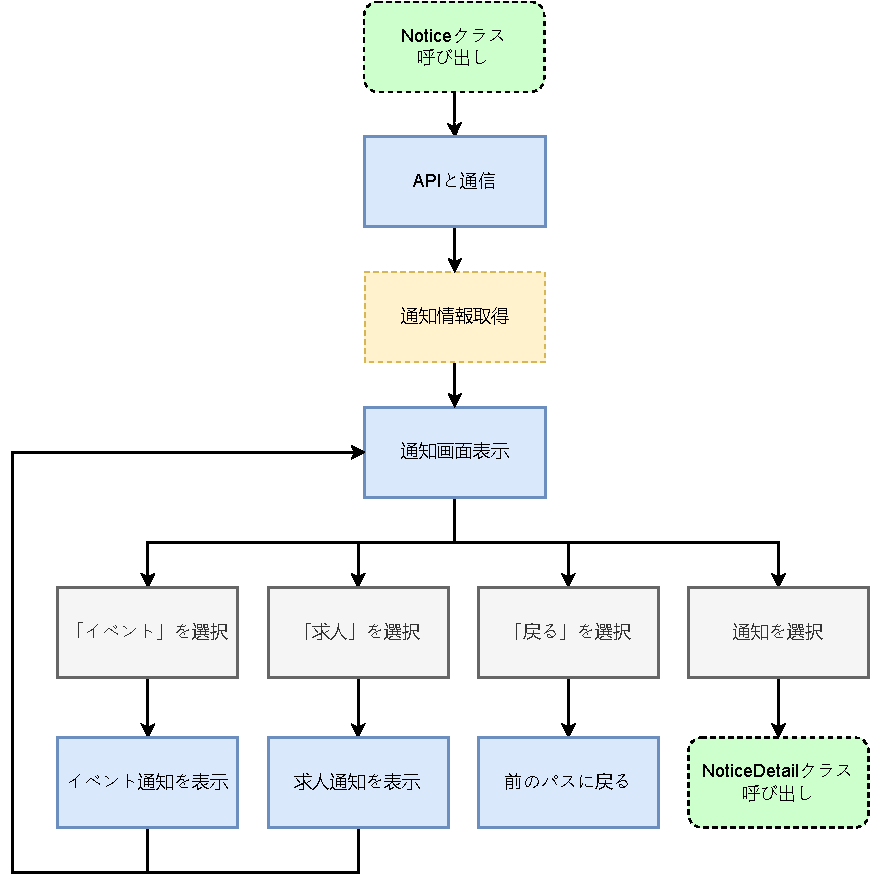
\includegraphics[scale = 0.9]{./images/internal-design/state_change_diagram/home/notice.pdf}
  \caption{notice.dartの状態遷移図}
\end{figure}

\begin{table}[H]
  \centering
  \begin{tabular}{|c|l|l|} \hline
    モジュール名                & \multicolumn{2}{l|}{notice\_detail.dart}                                                                                                                               \\ \hline
    モジュール概要               & \multicolumn{2}{p{12cm}|}{通知の詳細画面を表示するモジュール}                                                                                                                           \\ \hline
    責任者                   & \multicolumn{2}{l|}{新谷光城}                                                                                                                                              \\ \hline
    \multirow{7}{*}{構成要素} & クラス名                                         & NoticeDetail                                                                                                            \\ \cline{2-3}
                          & クラス種類                                        & extends StatelessWidget                                                                                                 \\ \cline{2-3}
                          & 処理概要                                         & \multicolumn{1}{p{12cm}|}{任意の通知詳細画面を生成するクラス}                                                                            \\ \cline{2-3}
                          & 入力                                           & \multicolumn{1}{p{12cm}|}{List$<$List$<$Map$<$String, dynamic$>$$>$$>$ titles, int is\_event, int index, String detail} \\ \cline{2-3}
                          & 出力                                           & Widget                                                                                                                  \\ \cline{2-3}
                          & \multicolumn{2}{l|}{他クラス・関数との関係}                                                                                                                                       \\ \cline{2-3}
                          & \multicolumn{2}{p{14cm}|}{
      titleAppBar.dartのTitleAppBarクラスを組み込む
      \newline noticeDetail.dartのNoticeContentクラスを組みむ
    \newline 戻るボタンの選択で前のモジュールに戻る}                                                                                                                                                                  \\ \hline
    \multirow{7}{*}{構成要素} & クラス名                                         & NoticeContent                                                                                                           \\ \cline{2-3}
                          & クラス種類                                        & extends StatelessWidget                                                                                                 \\ \cline{2-3}
                          & 処理概要                                         & \multicolumn{1}{p{12cm}|}{任意の通知内容のタイトルと本文を生成するクラス}                                                                      \\ \cline{2-3}
                          & 入力                                           & String title, String detail                                                                                             \\ \cline{2-3}
                          & 出力                                           & Widget                                                                                                                  \\ \cline{2-3}
                          & \multicolumn{2}{l|}{他クラス・関数との関係}                                                                                                                                       \\ \cline{2-3}
                          & \multicolumn{2}{p{14cm}|}{なし}                                                                                                                                          \\ \hline
  \end{tabular}
\end{table}

\begin{figure}[H]
  \centering
  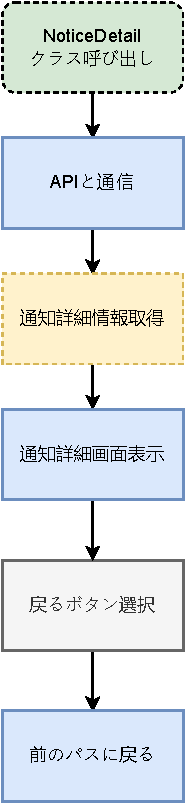
\includegraphics[scale = 0.9]{./images/internal-design/state_change_diagram/home/notice_detail.pdf}
  \caption{notice\_detail.dartの状態遷移図}
\end{figure}

\begin{table}[H]
  \centering
  \begin{tabular}{|c|l|l|} \hline
    モジュール名                & \multicolumn{2}{l|}{apply\_hist.dart}                                                            \\ \hline
    モジュール概要               & \multicolumn{2}{p{12cm}|}{応募を行った求人広告一覧を表示するモジュール}                                                \\ \hline
    責任者                   & \multicolumn{2}{l|}{新谷光城}                                                                        \\ \hline
    \multirow{7}{*}{構成要素} & クラス名                                              & ApplyHist                                    \\ \cline{2-3}
                          & クラス種類                                             & extends StatelessWidget                      \\ \cline{2-3}
                          & 処理概要                                              & \multicolumn{1}{p{12cm}|}{応募一覧画面を動的に変更するクラス} \\ \cline{2-3}
                          & 入力                                                & なし                                           \\ \cline{2-3}
                          & 出力                                                & Widget                                       \\ \cline{2-3}
                          & \multicolumn{2}{l|}{他クラス・関数との関係}                                                                 \\ \cline{2-3}
                          & \multicolumn{2}{p{14cm}|}{ApplyHistStateクラスを組み込む}                                                \\ \hline
    \multirow{7}{*}{構成要素} & クラス名                                              & ApplyHistState                               \\ \cline{2-3}
                          & クラス種類                                             & extends StatelessWidget                      \\ \cline{2-3}
                          & 処理概要                                              & \multicolumn{1}{p{12cm}|}{応募一覧画面の状態を返すクラス}   \\ \cline{2-3}
                          & 入力                                                & なし                                           \\ \cline{2-3}
                          & 出力                                                & State                                        \\ \cline{2-3}
                          & \multicolumn{2}{l|}{他クラス・関数との関係}                                                                 \\ \cline{2-3}
                          & \multicolumn{2}{p{14cm}|}{
      title\_appbar.dartのTitleAppBarクラスを組み込む
      \newline post\_list.dartのPostListクラスを組み込む
    \newline 戻るボタンの選択で前のモジュールに戻る}                                                                                            \\ \hline
  \end{tabular}
\end{table}

\begin{figure}[H]
  \centering
  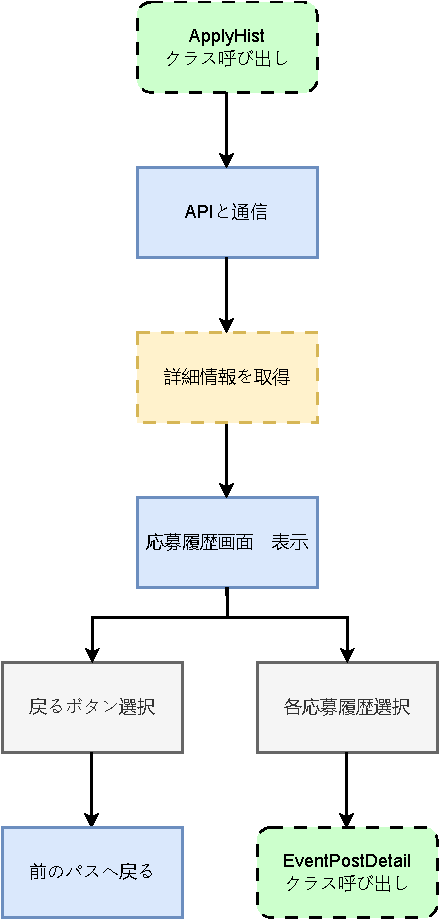
\includegraphics[scale = 0.8]{./images/internal-design/state_change_diagram/home/apply_hist.pdf}
  \caption{apply\_hist.dartの状態遷移図}
\end{figure}
\begin{table}[H]
  \centering
  \begin{tabular}{|c|l|l|} \hline
    モジュール名 & \multicolumn{2}{l|}{else\_list.dart} \\ \hline
    モジュール概要 & \multicolumn{2}{p{12cm}|}{イベント、求人の切り替えボタンのある一覧画面を表示} \\ \hline
    責任者 & \multicolumn{2}{l|}{新谷光城} \\ \hline
    \multirow{7}{*}{構成要素} & クラス名 & ElseList \\ \cline{2-3}
                            & クラス種類 & extends StatelessWidget \\ \cline{2-3}
                            & 処理概要 & \multicolumn{1}{p{12cm}|}{一覧画面を動的に変更するクラス} \\ \cline{2-3}
                            & 入力 & なし \\ \cline{2-3}
                            & 出力 & Widget \\ \cline{2-3}
                            & \multicolumn{2}{l|}{他クラス・関数との関係} \\ \cline{2-3}
                            & \multicolumn{2}{p{14cm}|}{else\_list.dartのElseListクラスを組み込む} \\ \hline
    \multirow{7}{*}{構成要素} & クラス名 & ElseListState \\ \cline{2-3}
                            & クラス種類 & extends StatelessWidget \\ \cline{2-3}
                            & 処理概要 & \multicolumn{1}{p{12cm}|}{一覧画面の状態を返す} \\ \cline{2-3}
                            & 入力 & なし \\ \cline{2-3}
                            & 出力 & State \\ \cline{2-3}
                            & \multicolumn{2}{l|}{他クラス・関数との関係} \\ \cline{2-3}
                            & \multicolumn{2}{p{14cm}|}{
                            change\_general\_corporation.dartのChangeGeneralCorporationプロバイダを組み込む
                            \newline title\_appbar.dartのTitleAppBarクラスを組み込む
                            \newline toggle\_button.dartのToggleButtonクラスを組み込む
                            \newline post\_list.dartのPostListクラスを組み込む} \\ \hline
  \end{tabular}
\end{table}

\begin{table}[H]
  \centering
  \begin{tabular}{|c|l|l|} \hline
    モジュール名 & \multicolumn{2}{l|}{event\_post\_detail.dart} \\ \hline
    モジュール概要 & \multicolumn{2}{p{12cm}|}{イベント広告詳細画面を表示するレイヤー} \\ \hline
    責任者 & \multicolumn{2}{l|}{新谷光城} \\ \hline
    \multirow{7}{*}{構成要素} & クラス名 & EventPostDetail \\ \cline{2-3}
                            & クラス種類 & extends StatelessWidget \\ \cline{2-3}
                            & 処理概要 & \multicolumn{1}{p{12cm}|}{イベント広告詳細画面を動的に変更するクラス} \\ \cline{2-3}
                            & 入力 & Map$<$String, dynamic$>$ info \\ \cline{2-3}
                            & 出力 & Widget \\ \cline{2-3}
                            & \multicolumn{2}{l|}{他クラス・関数との関係} \\ \cline{2-3}
                            & \multicolumn{2}{p{14cm}|}{event\_post\_detail.dartのEventPostDetailクラスを組み込む} \\ \hline
    \multirow{7}{*}{構成要素} & クラス名 & EventPostDetailState \\ \cline{2-3}
                            & クラス種類 & extends StatelessWidget \\ \cline{2-3}
                            & 処理概要 & \multicolumn{1}{p{12cm}|}{EventPostDetailState} \\ \cline{2-3}
                            & 入力 & なし \\ \cline{2-3}
                            & 出力 & State \\ \cline{2-3}
                            & \multicolumn{2}{l|}{他クラス・関数との関係} \\ \cline{2-3}
                            & \multicolumn{2}{p{14cm}|}{
                            change\_general\_corporation.dartのChangeGeneralCorporationプロバイダを組み込む
                            \newline title\_appbar.dartのTitleAppBarクラスを組み込む
                            \newline impression.dartのImpressionクラスを呼び出しインプレッション画面を表示
                            \newline event\_post\_write.dartのEventPostWriteクラスを呼び出しイベント広告内容変更画面を表示
                            \newline delete\_conf.dartのDeleteConfクラスを呼び出し投稿削除確認オーバーレイを表示} \\ \hline
  \end{tabular}
\end{table}

\begin{table}[H]
  \centering
  \begin{tabular}{|c|l|l|} \hline
    モジュール名 & \multicolumn{2}{l|}{event.dart} \\ \hline
    モジュール概要 & \multicolumn{2}{p{12cm}|}{イベント画面を表示するモジュール} \\ \hline
    責任者 & \multicolumn{2}{l|}{新谷光城} \\ \hline
    \multirow{7}{*}{構成要素} & クラス名 & EventRouterPage \\ \cline{2-3}
                            & クラス種類 & extends AppRouter \\ \cline{2-3}
                            & 処理概要 & \multicolumn{1}{p{12cm}|}{EventをアクセスするためのRouter} \\ \cline{2-3}
                            & 入力 & なし \\ \cline{2-3}
                            & 出力 & Route \\ \cline{2-3}
                            & \multicolumn{2}{l|}{他クラス・関数との関係} \\ \cline{2-3}
                            & \multicolumn{2}{p{14cm}|}{なし} \\ \hline
    \multirow{7}{*}{構成要素} & クラス名 & Event \\ \cline{2-3}
                            & クラス種類 & extends StatelessWidget \\ \cline{2-3}
                            & 処理概要 & \multicolumn{1}{p{12cm}|}{イベント画面を動的にするクラス} \\ \cline{2-3}
                            & 入力 & なし \\ \cline{2-3}
                            & 出力 & Widget \\ \cline{2-3}
                            & \multicolumn{2}{l|}{他クラス・関数との関係} \\ \cline{2-3}
                            & \multicolumn{2}{p{14cm}|}{event.dartのEventStateクラスを組み込む} \\ \hline
    \multirow{7}{*}{構成要素} & クラス名 & EventState \\ \cline{2-3}
                            & クラス種類 & extends StatelessWidget \\ \cline{2-3}
                            & 処理概要 & \multicolumn{1}{p{12cm}|}{イベント画面の状態を返すクラス} \\ \cline{2-3}
                            & 入力 & なし \\ \cline{2-3}
                            & 出力 & State \\ \cline{2-3}
                            & \multicolumn{2}{l|}{他クラス・関数との関係} \\ \cline{2-3}
                            & \multicolumn{2}{p{14cm}|}{
                            post\_list.dartのPostListクラスを組み込む
                            \newline else\_list.dartのElseListクラスを呼び出すことでお気に入りイベント一覧画面、閲覧履歴画面を表示
                            \newline search\_post.dartのSearchPostを呼び出すことで検索結果画面を表示
                            \newline event\_post\_write.dartのEventPostWriteクラスを呼び出すことでイベント詳細画面を表示} \\ \hline
  \end{tabular}
\end{table}

\begin{table}[H]
  \centering
  \begin{tabular}{|c|l|l|} \hline
    モジュール名 & \multicolumn{2}{l|}{posted\_list.dart} \\ \hline
    モジュール概要 & \multicolumn{2}{p{12cm}|}{法人利用者が投稿を行ったイベント、求人広告の一覧を表示するレイヤー} \\ \hline
    責任者 & \multicolumn{2}{l|}{新谷光城} \\ \hline
    \multirow{7}{*}{構成要素} & クラス名 & PostedList \\ \cline{2-3}
                            & クラス種類 & extends StatelessWidget \\ \cline{2-3}
                            & 処理概要 & \multicolumn{1}{p{12cm}|}{投稿一覧画面を動的に変更するクラス} \\ \cline{2-3}
                            & 入力 & なし \\ \cline{2-3}
                            & 出力 & Widget \\ \cline{2-3}
                            & \multicolumn{2}{l|}{他クラス・関数との関係} \\ \cline{2-3}
                            & \multicolumn{2}{p{14cm}|}{posted\_list.dartのPostedListStateクラスを組み込む} \\ \hline
    \multirow{7}{*}{構成要素} & クラス名 & PostedListState \\ \cline{2-3}
                            & クラス種類 & extends StatelessWidget \\ \cline{2-3}
                            & 処理概要 & \multicolumn{1}{p{12cm}|}{投稿一覧画面の状態を返すクラス} \\ \cline{2-3}
                            & 入力 & なし \\ \cline{2-3}
                            & 出力 & State \\ \cline{2-3}
                            & \multicolumn{2}{l|}{他クラス・関数との関係} \\ \cline{2-3}
                            & \multicolumn{2}{p{14cm}|}{
                            toggle\_button.dartのToggleButtonクラスを組み込む
                            \newline post\_list.dartのPostListクラスを組み込む
                            \newline event\_post\_write.dartのEventPostWriteクラスを呼び出すことでイベント詳細画面を表示
                            \newline job\_post\_write.dartのJobPostWriteクラスを呼び出すことで求人詳細画面を表示
                            \newline delete\_conf.dartのDeleteConfクラスを呼び出すことで削除確認オーバーレイを表示
                            \newline 戻るボタンの選択で前のレイヤーに戻る} \\ \hline
  \end{tabular}
\end{table}
\subsection*{component}

\begin{table}[H]
  \centering
  \begin{tabular}{|c|l|l|} \hline
    モジュール名 & \multicolumn{2}{l|}{post\_list.dart} \\ \hline
    モジュール概要 & \multicolumn{2}{p{12cm}|}{イベント、求人投稿の一覧を表示するレイヤー} \\ \hline
    責任者 & \multicolumn{2}{l|}{新谷光城} \\ \hline
    \multirow{7}{*}{構成要素} & クラス名 & PostList \\ \cline{2-3}
                            & クラス種類 & extends StatelessWidget \\ \cline{2-3}
                            & 処理概要 & \multicolumn{1}{p{12cm}|}{bodyの呼び出された部分に投稿一覧を設置するコンポーネント} \\ \cline{2-3}
                            & 入力 & List$<$Map$<$String, dynamic$>$$>$ articles, Map$<$String, dynamic$>$$>$ \\ \cline{2-3}
                            & 出力 & Widget \\ \cline{2-3}
                            & \multicolumn{2}{l|}{他クラス・関数との関係} \\ \cline{2-3}
                            & \multicolumn{2}{p{14cm}|}{
                            event\_post\_detail.dartのEventPostDetailクラスを呼び出すことでイベント広告詳細画面を表示
                            \newline job\_post\_detail.dartのJobPostDetailクラスを呼び出すことでイベント広告詳細画面を表示} \\ \hline
  \end{tabular}
\end{table}

\begin{table}[H]
  \centering
  \begin{tabular}{|c|l|l|} \hline
    モジュール名 & \multicolumn{2}{l|}{text\_enter\_box.dart} \\ \hline
    モジュール概要 & \multicolumn{2}{p{12cm}|}{デコレーションされた入力フォームを返すコンポーネント} \\ \hline
    責任者 & \multicolumn{2}{l|}{山本昇永} \\ \hline
    \multirow{7}{*}{構成要素} & クラス名 & TextEnterBox \\ \cline{2-3}
                            & クラス種類 & extends StatelessWidget \\ \cline{2-3}
                            & 処理概要 & \multicolumn{1}{p{12cm}|}{入力フォームを表示するクラス} \\ \cline{2-3}
                            & 入力 & String label, String histText, double width, bool isShow \\ \cline{2-3}
                            & 出力 & Widget \\ \cline{2-3}
                            & \multicolumn{2}{l|}{他クラス・関数との関係} \\ \cline{2-3}
                            & \multicolumn{2}{p{14cm}|}{なし} \\ \hline
  \end{tabular}
\end{table}

\begin{table}[H]
  \centering
  \begin{tabular}{|c|l|l|} \hline
    モジュール名 & \multicolumn{2}{l|}{password\_input.dart} \\ \hline
    モジュール概要 & \multicolumn{2}{p{12cm}|}{パスワードを入力するフォームを作成するコンポーネント} \\ \hline
    責任者 & \multicolumn{2}{l|}{山本昇永} \\ \hline
    \multirow{7}{*}{構成要素} & クラス名 & PasswordInput \\ \cline{2-3}
                            & クラス種類 & extends StatelessWidget \\ \cline{2-3}
                            & 処理概要 & \multicolumn{1}{p{12cm}|}{パスワード入力フォームのWidgetを動的に変更するクラス} \\ \cline{2-3}
                            & 入力 & String label, bool isHidden \\ \cline{2-3}
                            & 出力 & Widget \\ \cline{2-3}
                            & \multicolumn{2}{l|}{他クラス・関数との関係} \\ \cline{2-3}
                            & \multicolumn{2}{p{14cm}|}{password\_input.dartのPasswordInputStateクラスを読み込む} \\ \hline
    \multirow{7}{*}{構成要素} & クラス名 & PasswordInputState \\ \cline{2-3}
                            & クラス種類 & extends State \\ \cline{2-3}
                            & 処理概要 & \multicolumn{1}{p{12cm}|}{パスワード入力フォームの状態を返すクラス} \\ \cline{2-3}
                            & 入力 & なし \\ \cline{2-3}
                            & 出力 & State \\ \cline{2-3}
                            & \multicolumn{2}{l|}{他クラス・関数との関係} \\ \cline{2-3}
                            & \multicolumn{2}{p{14cm}|}{なし} \\ \hline
  \end{tabular}
\end{table}

\begin{table}[H]
  \centering
  \begin{tabular}{|c|l|l|} \hline
    モジュール名 & \multicolumn{2}{l|}{company\_form.dart} \\ \hline
    モジュール概要 & \multicolumn{2}{p{12cm}|}{法人が入力するフォームを出力するコンポーネント} \\ \hline
    責任者 & \multicolumn{2}{l|}{山本昇永} \\ \hline
    \multirow{7}{*}{構成要素} & クラス名 & CompanyForm \\ \cline{2-3}
                            & クラス種類 & extends StatelessWidget \\ \cline{2-3}
                            & 処理概要 & \multicolumn{1}{p{12cm}|}{法人用の入力フォームのWidgetを動的に変更するクラス} \\ \cline{2-3}
                            & 入力 & bool canEdit \\ \cline{2-3}
                            & 出力 & Widget \\ \cline{2-3}
                            & \multicolumn{2}{l|}{他クラス・関数との関係} \\ \cline{2-3}
                            & \multicolumn{2}{p{14cm}|}{なし} \\ \hline
    \multirow{7}{*}{構成要素} & クラス名 & CompanyFormState \\ \cline{2-3}
                            & クラス種類 & extends State \\ \cline{2-3}
                            & 処理概要 & \multicolumn{1}{p{12cm}|}{法人用の入力フォームの状態を返すクラス} \\ \cline{2-3}
                            & 入力 & なし \\ \cline{2-3}
                            & 出力 & State \\ \cline{2-3}
                            & \multicolumn{2}{l|}{他クラス・関数との関係} \\ \cline{2-3}
                            & \multicolumn{2}{p{14cm}|}{text\_enter\_box.dartのTextEnterBoxクラスを呼び出すことで入力フォームを表示} \\ \hline
  \end{tabular}
\end{table}

\begin{table}[H]
  \centering
  \begin{tabular}{|c|l|l|} \hline
    モジュール名 & \multicolumn{2}{l|}{finish\_screen.dart} \\ \hline
    モジュール概要 & \multicolumn{2}{p{12cm}|}{完了画面を生成するコンポーネント} \\ \hline
    責任者 & \multicolumn{2}{l|}{金川幸太} \\ \hline
    \multirow{7}{*}{構成要素} & クラス名 & FinishScreen \\ \cline{2-3}
                            & クラス種類 & extends StatelessWidget \\ \cline{2-3}
                            & 処理概要 & \multicolumn{1}{p{12cm}|}{アイコン、テキストを引数で与えることによって、任意の完了画面を生成するコンポーネント} \\ \cline{2-3}
                            & 入力 & \multicolumn{1}{p{12cm}|}{String appbarText, IconData appIcon, String text, String buttonText bool isAppbar} \\ \cline{2-3}
                            & 出力 & Widget \\ \cline{2-3}
                            & \multicolumn{2}{l|}{他クラス・関数との関係} \\ \cline{2-3}
                            & \multicolumn{2}{p{14cm}|}{
                              title\_appbar.dartのTitleAppBarクラスを組み込む
                              \newline normal\_bottom\_appbar.dartのNormalBottomAppBarクラスを組み込む
                              \newline button\_set.dartのButtonSetクラスを組み込む
                              \newline LoginRouteの最初の画面へと戻る
                            } \\ \hline
    \multirow{7}{*}{構成要素} & クラス名 & QuestionButton \\ \cline{2-3}
                            & クラス種類 & extends StatelessWidget \\ \cline{2-3}
                            & 処理概要 & \multicolumn{1}{p{12cm}|}{お問合せボタンを生成するコンポーネント} \\ \cline{2-3}
                            & 入力 & なし \\ \cline{2-3}
                            & 出力 & Widget \\ \cline{2-3}
                            & \multicolumn{2}{l|}{他クラス・関数との関係} \\ \cline{2-3}
                            & \multicolumn{2}{p{14cm}|}{
                            change\_general\_corporation.dartのChangeGeneralCorporationクラスを組み込む
                            \newline ask\_page.dartのAskPageクラスを呼び出し問い合わせ画面を表示} \\ \hline
  \end{tabular}
\end{table}

\begin{table}[H]
  \centering
  \begin{tabular}{|c|l|l|} \hline
    モジュール名 & \multicolumn{2}{l|}{coment\_box.dart} \\ \hline
    モジュール概要 & \multicolumn{2}{p{12cm}|}{コメントまたは文を入力できる項目を生成するコンポーネント} \\ \hline
    責任者 & \multicolumn{2}{l|}{金川幸太} \\ \hline
    \multirow{7}{*}{構成要素} & クラス名 & ComentBox \\ \cline{2-3}
                            & クラス種類 & extends StatelessWidget \\ \cline{2-3}
                            & 処理概要 & \multicolumn{1}{p{12cm}|}{このクラスはbodyで呼び出された箇所にコメントボックスを生成する} \\ \cline{2-3}
                            & 入力 & int boxWidth, int boxHeight \\ \cline{2-3}
                            & 出力 & Widget \\ \cline{2-3}
                            & \multicolumn{2}{l|}{他クラス・関数との関係} \\ \cline{2-3}
                            & \multicolumn{2}{p{14cm}|}{なし} \\ \hline
  \end{tabular}
\end{table}

\begin{table}[H]
  \centering
  \begin{tabular}{|c|l|l|} \hline
    モジュール名 & \multicolumn{2}{l|}{button\_set.dart} \\ \hline
    モジュール概要 & \multicolumn{2}{p{12cm}|}{任意のテキストが書かれたボタンを生成するレイヤー} \\ \hline
    責任者 & \multicolumn{2}{l|}{金川幸太} \\ \hline
    \multirow{7}{*}{構成要素} & クラス名 & ButtonSet \\ \cline{2-3}
                            & クラス種類 & extends StatelessWidget \\ \cline{2-3}
                            & 処理概要 & \multicolumn{1}{p{12cm}|}{bodyの呼び出された部分にボタンを設置するコンポーネント} \\ \cline{2-3}
                            & 入力 & Sting buttonName \\ \cline{2-3}
                            & 出力 & Widget \\ \cline{2-3}
                            & \multicolumn{2}{l|}{他クラス・関数との関係} \\ \cline{2-3}
                            & \multicolumn{2}{p{14cm}|}{change\_general\_corporation.dartのChangeGeneralCorporationクラスを組み込む} \\ \hline
  \end{tabular}
\end{table}

\begin{table}[H]
  \centering
  \begin{tabular}{|c|l|l|} \hline
    モジュール名 & \multicolumn{2}{l|}{toggle\_button.dart} \\ \hline
    モジュール概要 & \multicolumn{2}{p{12cm}|}{二つの条件を切り替えるtoggleButtonを作成するレイヤー} \\ \hline
    責任者 & \multicolumn{2}{l|}{新谷光城} \\ \hline
    \multirow{7}{*}{構成要素} & クラス名 & ChangeToggleButton \\ \cline{2-3}
                            & クラス種類 & ChangeNotifier \\ \cline{2-3}
                            & 処理概要 & \multicolumn{1}{p{12cm}|}{ToggleButtonにて使用するボタンが押されているか否かを判定するbool型の変数
                            とその変数の値を変更する関数を定義するプロバイダ} \\ \cline{2-3}
                            & 入力 & なし \\ \cline{2-3}
                            & 出力 & Widget \\ \cline{2-3}
                            & \multicolumn{2}{l|}{他クラス・関数との関係} \\ \cline{2-3}
                            & \multicolumn{2}{p{14cm}|}{なし} \\ \hline
    \multirow{7}{*}{構成要素} & クラス名 & ToggleButton \\ \cline{2-3}
                            & クラス種類 & extends StatelessWidget \\ \cline{2-3}
                            & 処理概要 & \multicolumn{1}{p{12cm}|}{二つの条件を切り替えるToggleButtonを作成するWidgetを返す} \\ \cline{2-3}
                            & 入力 & \multicolumn{1}{p{12cm}|}{
                            MediaQueryData mediaQuery, String leftName, String rightName, double buttonHeight} \\ \cline{2-3}
                            & 出力 & Widget \\ \cline{2-3}
                            & \multicolumn{2}{l|}{他クラス・関数との関係} \\ \cline{2-3}
                            & \multicolumn{2}{p{14cm}|}{
                              toggleButton.dartのChangeToggleButtonクラスを組み込む
                              \newline change\_general\_corporation.dartのChangeGeneralCorporationクラスを組み込む
                            } \\ \hline
  \end{tabular}
\end{table}

\begin{table}[H]
  \centering
  \begin{tabular}{|c|l|l|} \hline
    モジュール名 & \multicolumn{2}{l|}{normal\_bottom\_appbar.dart} \\ \hline
    モジュール概要 & \multicolumn{2}{p{12cm}|}{BottomNavigationBarがない画面で用いるBottomAppBarを作成するコンポーネント} \\ \hline
    責任者 & \multicolumn{2}{l|}{新谷光城} \\ \hline
    \multirow{7}{*}{構成要素} & クラス名 & NormalBottomAppBar \\ \cline{2-3}
                            & クラス種類 & extends StatelessWidget \\ \cline{2-3}
                            & 処理概要 & \multicolumn{1}{p{12cm}|}{色がついただけのBottomAppBarのWidgetを返すコンポーネント} \\ \cline{2-3}
                            & 入力 & なし \\ \cline{2-3}
                            & 出力 & Widget \\ \cline{2-3}
                            & \multicolumn{2}{l|}{他クラス・関数との関係} \\ \cline{2-3}
                            & \multicolumn{2}{p{14cm}|}{なし} \\ \hline
  \end{tabular}
\end{table}

\begin{table}[H]
  \centering
  \begin{tabular}{|c|l|l|} \hline
    モジュール名 & \multicolumn{2}{l|}{title\_appbar.dart} \\ \hline
    モジュール概要 & \multicolumn{2}{p{12cm}|}{AppBarの下にページタイトルを表示するAppBarを作成するコンポーネント} \\ \hline
    責任者 & \multicolumn{2}{l|}{新谷光城} \\ \hline
    \multirow{7}{*}{構成要素} & クラス名 & TitleAppBar \\ \cline{2-3}
                            & クラス種類 & extends StatelessWidget \\ \cline{2-3}
                            & 処理概要 & \multicolumn{1}{p{12cm}|}{AppBarのbottomにてもう一度AppBarを作成し、そこにページのタイトルを表示させるAppBarを生成するコンポーネント} \\ \cline{2-3}
                            & 入力 & String appbarText, bool isReturn \\ \cline{2-3}
                            & 出力 & Widget \\ \cline{2-3}
                            & \multicolumn{2}{l|}{他クラス・関数との関係} \\ \cline{2-3}
                            & \multicolumn{2}{p{14cm}|}{popを行う} \\ \hline
  \end{tabular}
\end{table}


\section{API設計}\label{sec:api}
\subsection*{認証}
\subsubsection*{ログイン}
\textbf{POST} \texttt{auth/login} \\
\begin{table}[H]
  \begin{minipage}
    {0.5\hsize} \centering
    \captionsetup{labelformat=empty,labelsep=none}
    \caption{\textbf{Request}}
    \begin{tabular}{|c|c|c|} \hline
      パラメータ    & 型      & 説明    \\ \hline \hline
      username & string & ユーザ名  \\ \hline
      password & string & パスワード \\ \hline
    \end{tabular}
  \end{minipage}
  \begin{minipage}
    {0.5\hsize} \centering
    \captionsetup{labelformat=empty,labelsep=none}
    \caption{\textbf{Response}}
    \begin{tabular}{|c|c|c|} \hline
      パラメータ & 型      & 説明    \\ \hline \hline
      token & string & トークン  \\ \hline
      user  & object & ユーザ情報 \\ \hline
    \end{tabular}
  \end{minipage}
\end{table}

\subsubsection*{ログアウト}
\textbf{POST} \texttt{auth/logout} \\
\begin{table}[H]
  \begin{minipage}
    {0.5\hsize} \centering
    \captionsetup{labelformat=empty,labelsep=none}
    \caption{\textbf{Request}}
    \begin{tabular}{|c|c|c|} \hline
      パラメータ & 型      & 説明   \\ \hline \hline
      token & string & トークン \\ \hline
    \end{tabular}
  \end{minipage}
  \begin{minipage}
    {0.5\hsize} \centering
    \captionsetup{labelformat=empty,labelsep=none}
    \caption{\textbf{Response}}
    \begin{tabular}{|c|c|c|} \hline
      パラメータ   & 型      & 説明    \\ \hline \hline
      message & string & メッセージ \\ \hline
    \end{tabular}
  \end{minipage}
\end{table}

\subsubsection*{ユーザ登録}

\section{データベース設計}
以下に、本アプリケーションにおけるデータベース設計を示す。
なお、都合上Userテーブルへの接続について分割を行っている。
\begin{figure}[H]
  \centering
  
\includegraphics[width=15cm]{./images/internal-design/ER-1.pdf}
  \caption{ER図(1)}
  \label{fig:ER1}
\end{figure}
\begin{figure}[H]
  \centering
  
\includegraphics[width=15cm]{./images/internal-design/ER-2.pdf}
  \caption{ER図(2)}
  \label{fig:ER2}
\end{figure}
\section{各メンバーの貢献度}
\begin{thebibliography}{1}
  \bibitem{bib:pep8}
  ``PEP8-Style Guide for Python Code,''\\
  \url{https://peps.python.org/pep-0008/}, 2023/12/5 閲覧.
\end{thebibliography}
\end{document}